\newpage
\section{HÀM SỐ BẬC HAI. ĐỒ THỊ HÀM SỐ BẬC HAI VÀ ỨNG DỤNG}
\subsection{LÝ THUYẾT CẦN NHỚ}
\subsubsection{Hàm số bậc hai}
\indam{Định nghĩa:}
\begin{boxdn}
	\textit{Hàm số bậc hai theo biến $ x $} là hàm số được cho bằng biểu thức có dạng $y = ax^2 + bx + c$, trong đó $a$, $b$, $c$ là những hằng số và $a$ khác $0$. Tập xác định của hàm số là $\mathbb{R}$.
\end{boxdn}

\subsubsection{Đồ thị hàm số bậc hai}
\begin{boxdn}
	\begin{itemize}
		\item \textit{Đồ thị hàm số bậc hai} $y = ax^{2} + bx + c$ $(a \neq 0)$ là một đường parabol có đỉnh là điểm với toạ độ $\left(-\dfrac{b}{2a};-\dfrac{\Delta}{4a}\right)$ và trục đối xứng là đường thẳng $x=-\dfrac{b}{2a}$.
		\item \textit{Nhận xét.} Cho hàm số $f(x)=a x^2+b x+c$ $(a \neq 0)$, ta có $-\dfrac{\Delta}{4 a}=f\left(\dfrac{-b}{2 a}\right)$.
	\end{itemize}
\end{boxdn}

%-------------------------------------------------------------------------------------------------------------
\subsection{PHÂN LOẠI VÀ PHƯƠNG PHÁP GIẢI TOÁN}
\begin{dang}{Xác định công thức hàm số bậc hai}
	\textit{Phương pháp:} Sử dụng kiến thức
	\begin{itemize}
		\item $ f(x)=ax^2+bx+c $ là hàm số bậc hai khi $ a\ne 0 $.
		\item Đồ thị hàm số bậc hai $ (P)\colon y=ax^2+bx+c $ có đỉnh $ I(x_I;y_I)$ thì $\heva{&I \in (P)\\&x=-\dfrac{b}{2a}.}$
		\item Điểm $M(x_0; y_0)$ thuộc đồ thị hàm số $y = ax^2 + bx + c$ nếu $y_0 = ax_0^2 + bx_0 + c$.
	\end{itemize}

\end{dang}
\begin{vd}%[0D3N2-1]%[Dự án đề cương 2025]%[Đoàn Minh Tâm]
	Tìm tất cả các số thực $ m $ để các hàm số sau là hàm số bậc hai.
	\begin{enumerate}
		\item $ f(x)=(m^2-1)x^2+2(m-1)x+3 $.
		\item $ g(x)=(m^2-m-6)x^3+(3-m)x^2-6x+m $.
	\end{enumerate}
	\loigiai{
		\begin{enumerate}
			\item Ta có $ f(x) $ là hàm số bậc hai khi và chỉ khi
			$$ m^2-1 \ne 0 \Leftrightarrow m\ne \pm 1. $$
			\item Ta có $ g(x) $ là hàm số bậc hai khi và chỉ khi
			$$ \heva{&m^2-m-6 =0\\&3-m\ne 0}\Leftrightarrow \heva{&\hoac{&m=-2\\&m=3}\\&m\ne 3}\Leftrightarrow m=-2. $$
		\end{enumerate}
}
\end{vd}

\begin{vd}%[0D3H2-1]%[Dự án đề cương 2025]%[Đoàn Minh Tâm]
	\begin{enumerate}
		\item Xác định parabol $y=ax^2+bx+3$, biết rằng parabol đi qua hai điểm $A(1;2)$ và $B(-2;11)$.
		\item Xác định parabol có đỉnh $I(1 ; 2)$ và đi qua điểm $M(0 ; 3)$.
	\end{enumerate}

	\loigiai{
		\begin{enumerate}
		\item 	Parabol $(P)\colon y=ax^2+bx+3$ $(a \ne 0)$.
		Vì $(P)$ đi qua $A(1;2)$ nên $2=a+b+3 \Leftrightarrow a+b=-1.\quad(1)$\\
		Vì $(P)$ đi qua $B(-2;11)$ nên $11=4a-2b+3 \Leftrightarrow 4a-2b=8.\quad(2)$\\
		Từ $(1)$ và $(2)$ ta có $\heva{&a+b=-1\\&4a-2b=8} \Leftrightarrow \heva{&a=1\\&b=-2.}$\\
		Vậy parabol $(P)\colon y=x^2-2x+3$.
			\item Gọi hàm số bậc hai có parabol thoả mãn đề bài là $y = ax^{2} + bx + c\ (a \neq 0)$.\\
			Parabol đi qua $M(0 ; 3)$ nên ta có: $0^{2} a+0 b+c=3$. Do đó, $c=3$.\\
			Parabol có đỉnh $I(1 ; 2)$ nên ta có $\heva{&-\dfrac{b}{2a} = 1\\& a + b + 3 = 2} \Leftrightarrow \heva{&b = -2a \\& a + b = -1} \Leftrightarrow \heva{&a = 1 \\& b = -2.}$\\
			Vậy parabol cần tìm là $y=x^{2}-2 x+3$.\\
			\begin{nx}
				Giả thiết parabol có đỉnh $I(1 ; 2)$ trong bài tập có thể thay bằng một số cách phát biểu sau đây:
				\begin{itemize}
					\item Parabol có trục đối xứng $x=1$ và đi qua điểm $I(1 ; 2)$.
					\item Parabol có trục đối xứng $x=1$ và tung độ của điểm thấp nhất bằng $2$.
					\item Parabol đi qua điểm $I(1 ; 2)$ và tung độ của điểm thấp nhất bằng $2$.
					\item Parabol có trục đối xứng $x=1$ và có tung độ đỉnh là $2$.
				\end{itemize}
			\end{nx}
		\end{enumerate}

	}
\end{vd}
\begin{dang}{Sự biến thiên của hàm số bậc hai}
\begin{itemize}
	\item \textit{Phương pháp:} Áp dụng bảng biến thiên của hàm số bậc hai $y = ax^2 + bx + c$:
	\begin{center}
		\newcolumntype{C}{>{\centering\arraybackslash}p{7.5cm}}
		\begin{tabular}{CC}
			$a>0$ & $a<0$\\
			
\begin{tikzpicture}[>=stealth,scale=1]
				\tkzTabInit[lgt=1,espcl=2.5]
				{$x$ /1, $y$ /2}
				{$-\infty$,$-\dfrac{b}{2a}$,$\infty$}
				\tkzTabVar{+/$+\infty$,-/$-\dfrac{\Delta}{4a}$,+/$+\infty$}
			\end{tikzpicture}
			&
			
\begin{tikzpicture}[>=stealth,scale=1]
				\tkzTabInit[lgt=1,espcl=2.5]
				{$x$ /1, $y$ /2}
				{$-\infty$,$-\dfrac{b}{2a}$,$\infty$}
				\tkzTabVar{-/$-\infty$,+/$-\dfrac{\Delta}{4a}$,-/$-\infty$}
			\end{tikzpicture}\\
		\end{tabular}
	\end{center}
\end{itemize}
\end{dang}
\begin{vd}%[0D3H2-2]%[Dự án đề cương 2025]%[Đoàn Minh Tâm]
	Cho hàm số $y=f(x)=2 x^2+4x-2$.
	\begin{enumerate}
		 \item Lập bảng biến thiên của hàm số $y=f(x)$.
		 \item Xác định khoảng đồng biến và khoảng nghịch biến của hàm số trên.
		 \item Xác định tập giá trị của hàm số $ f(x) $.
	\end{enumerate}
	\loigiai{
			\begin{enumerate}
				\item Ta có $a=2>0$, $b=4$, $-\dfrac{b}{2 a}=-1$. Vậy ta có bảng biến thiên của hàm số $y=f(x)$ như sau
				\begin{center}
						
\begin{tikzpicture}[>=stealth,scale=1]
						\tkzTabInit[lgt=1,espcl=2.5]
						{$x$ /1, $y$ /1.6}
						{$-\infty$,$-1$,$\infty$}
						\tkzTabVar{+/$+\infty$,-/$-4$,+/$+\infty$}
					\end{tikzpicture}
				\end{center}
				\item Hàm số đồng biến trên khoảng $(-1 ;+\infty)$ và nghịch biến trên khoảng $(-\infty ;-1)$.
				\item Dựa vào bảng biến thiên ta có tập giá trị là $ T=[-4;+\infty] $.
			\end{enumerate}
	}
\end{vd}

\begin{dang}{Đồ thị hàm số bậc hai (parabol)}
		\begin{itemize}
		\item Cách vẽ đồ thị hàm số bậc hai $y=ax^2+bx+c$ (với $a\ne 0$):
		\begin{enumerate}
			\item Xác định tọa độ đỉnh $S\left(-\dfrac{b}{2a};-\dfrac{\Delta}{4a}\right)$.
			\item Vẽ trục đối xứng $d$ là đường thẳng $x=-\dfrac{b}{2a}$.
			\item Tìm tọa độ giao điểm của đồ thị với trục tung (điểm $A(0;c)$) và giao điểm của đồ thị với trục hoành (nếu có).\\
			Xác định thêm điểm đối xứng với $A$ qua trục đối xứng $d$, là điểm $B\left(-\dfrac{b}{a};c\right)$.
			\item Vẽ parabol có đỉnh $S$, có trục đối xứng $d$, đi qua các điểm tìm được.
		\end{enumerate}
		\item \textit{Chú ý:} Nếu $a>0$ thì parabol có bề lõm quay lên trên, nếu $a<0$ thì parabol có bề lõm quay xuống dưới.
	\end{itemize}
\end{dang}
\begin{vd}%[0D3H2-3]%[Dự án đề cương 2025]%[Đoàn Minh Tâm]
	Vẽ đồ thị các hàm số:
	\begin{enumerate}
		\item $y=f(x)=-x^2+4x-3$;
		\item $y=f(x)=x^2+2x+2$.
	\end{enumerate}
	\loigiai{
		\begin{enumerate}
			\item Trong mặt phẳng tọa độ $Oxy$, đồ thị hàm số bậc hai $y=f(x)=-x^2+4x-3$ là một parabol $(P)$:
			\immini{
				\begin{itemize}
					\item Có đỉnh $S(2;1)$;
					\item Có trục đối xứng là đường thẳng $x=2$ (đường thẳng này đi qua đỉnh $S$ và song song với trục $Oy$);
					\item Bề lõm quay xuống dưới vì $a<0$;
					\item Cắt trục tung tại điểm có tung độ bằng $-3$, tức là đồ thị đi qua điểm có tọa độ $(0;-3)$.\\
					Ngoài ra, phương trình $-x^2+4x-3=0$ có hai nghiệm phân biệt $x_1=1$ và $x_2=3$ nên đồ thị hàm số cắt trục hoành tại hai điểm có tọa độ $(1;0)$ và $(3;0)$.\\
					Ta vẽ được đồ thị như hình bên.
				\end{itemize}
			}{
				\begin{tikzpicture}[scale=0.7, font=\footnotesize, line join=round, line cap=round, >=stealth]
					\draw [->] (-1,0)--(6,0) node[below]{$x$};
					\draw [->] (0,-6)--(0,3) node[right]{$y$};
					\draw[fill=black] (0,0) circle(1pt) node[below left]{$O$};
					\clip (-1,-6) rectangle (6,3);
					\draw[smooth, samples=300, domain=-1:5] plot (\x,{-1*(\x)^2+4*(\x)-3});
					\draw[dashed] (0,1)--(2,1);
					\draw[fill=black] (2,1) circle(1pt)node[above right]{$S(2;1)$};
					\draw[fill=black] (1,0) circle(1pt)node[below]{$1$};
					\draw [fill=black](3,0) circle(1pt)node[below]{$3$};
					\draw (2,-4) node[right]{$x=2$};
					\draw[dashed] (2,-6)--(2,3);
					\draw[fill=black] (2,0) circle(1pt) node[below right]{$2$};
					\draw[fill=black] (4,0) circle(1pt) node[below]{$4$};
					\draw[fill=black] (0,1) circle(1pt) node[left]{$1$};
					\draw[fill=black] (0,-3) circle(1pt) node[left]{$-3$};
				\end{tikzpicture}
			}
			\item Trong mặt phẳng tọa độ $Oxy$, đồ thị hàm số bậc hai $y=f(x)=x^2+2x+2$ là một parabol $(P)$.
			\immini{
				\begin{itemize}
					\item Có đỉnh $S(-1;1)$;
					\item Có trục đối xứng là đường thẳng $x=-1$ (đường thẳng này đi qua đỉnh $S$ và song song với trục $Oy$);
					\item Bề lõm quay lên trên vì $a>0$;
					\item Cắt trục tung tại điểm có tung độ bằng $2$, tức là đồ thị đi qua điểm có tọa độ $(0;2)$.\\
					Ta vẽ được đồ thị như hình bên.
				\end{itemize}
			}{
				\begin{tikzpicture}[scale=0.8, font=\footnotesize, line join=round, line cap=round, >=stealth]
					\draw [->] (-4,0)--(3,0) node[below]{$x$};
					\draw [->] (0,-1.5)--(0,6) node[left]{$y$};
					\draw[fill=black] (0,0) circle(1pt) node[below right]{$O$};
					\clip (-4,-1.5) rectangle (3,6);
					\draw[smooth, samples=300, domain=-4:2] plot (\x,{(\x)^2+2*(\x)+2});
					\draw[dashed] (0,1)--(-1,1);
					\draw[fill=black] (-1,1) circle(1pt)node[below left]{$S(-1;1)$};
					\draw (-1,-1.2) node[left]{$x=-1$};
					\draw[dashed] (-1,-1.5)--(-1,6);
					\foreach \i in {-3,-2,1,2} \draw[fill=black] (\i,0) circle(1pt) node[below]{$\i$};
					\foreach \j in {-1,2,3,4,5} \draw[fill=black] (0,\j) circle(1pt) node[left]{$\j$};
					\draw[fill=black] (-1,0) circle(1pt) node[below right]{$-1$};
					\draw[fill=black] (0,1) circle(1pt) node[right]{$1$};
					\draw (0,2) node[right]{$(0;2)$};
				\end{tikzpicture}
			}
		\end{enumerate}
	}%<MyLT2>
\end{vd}

\begin{vd}%[0D3H2-3]%[Dự án đề cương 2025]%[Đoàn Minh Tâm]
	\immini{Cho hàm số $y=a x^2+b x+c$ có đồ thị ở hình bên. Xác định dấu của $a$, $b$ và $c$.}{
		\begin{tikzpicture}[scale=0.8, font=\footnotesize, line join=round, line cap=round, >=stealth]
			\def\hso{\x*\x-3*\x+1.5}
			\draw[thick,samples=200,smooth]plot[domain=-.5:3.5](\x,{\hso});
			\draw[->](-1,0)--(5,0)node[below left]{$x$};
			\draw[->](0,-1)--(0,4)node[below left]{$y$};
			\foreach \i in {1,...,4}{\draw (\i,.1)--(\i,-.1);}
			\foreach \i in {1,...,3}{\draw (.1,\i)--(-.1,\i);}
			\path (0,0) node[below left]{$O$};
		\end{tikzpicture}
	}
	\loigiai{
		\immini{
			Parabol hướng bề lõm lên trên nên $a>0$.\\
			Parabol cắt trục tung tại điểm $(0 ; c)$ nằm phía trên trục hoành nên $c>0$.\\
			Đỉnh nằm bên phải trục tung nên hoành độ đỉnh dương hay $\dfrac{-b}{2 a}>0$.\\
			Do $a>0$ nên $b<0$.\\
			Vậy $a>0$, $b<0$ và $c>0$.
		}{
		\begin{tikzpicture}[scale=0.8, font=\footnotesize, line join=round, line cap=round, >=stealth]
			\def\hso{\x*\x-3*\x+1.5}
			\draw[thick,samples=200,smooth]plot[domain=-.5:3.5](\x,{\hso});
			\draw[->](-1,0)--(5,0)node[below left]{$x$};
			\draw[->](0,-1)--(0,4)node[below left]{$y$};
			\foreach \i in {1,...,4}{\draw (\i,.1)--(\i,-.1);}
			\foreach \i in {1,...,3}{\draw (.1,\i)--(-.1,\i);}
			\path (0,0) node[below left]{$O$};
		\end{tikzpicture}
		}
	}
\end{vd}
\begin{dang}{Ứng dụng hàm số bậc hai để giải các bài toán thực tế}
	\textbf{Phương pháp giải:} Mô hình hóa bài toán về phương trình hàm số bậc hai hoặc ứng dụng đồ thị hàm số bậc hai để giải quyết các bài toán thực tế
\end{dang}

\begin{vd}%[0D3V2-6]%[Dự án đề cương 2025]%[Đoàn Minh Tâm]
	\immini{
		Tại một buổi khai trương, người ta làm một cổng chào có đường viền trong của mặt cắt là đường parabol. Người ta đo khoảng cách giữa hai chân cổng là $4{,}5$ m. Từ một điểm trên thân cổng người ta đo được khoảng cách tới mặt đất là $1{,}8$ m và khoảng cách từ điểm đó tới chân cổng gần nhất là $1$ m. Hãy tính chiều cao của cổng chào đó (tính theo đường viền trong) theo đơn vị mét và làm tròn kết quả đển hàng phần mười.
	}{
		\begin{tikzpicture}[scale=1.2, font=\footnotesize, line join=round, line cap=round, >=stealth]
			\def\hso{-18/35*\x*\x+81/35*\x}
			\def\hsoo{-18/35*\x*\x+81/35*\x+.75}
			\draw[thick,blue,samples=200,smooth,fill=gray,xscale=1.2]plot[domain=0:4.5](\x,{\hso})--cycle;
			\draw[thick,blue,samples=200,smooth,fill=white,xscale=1.2]plot[domain=0:4.5](\x,{\hsoo})--cycle;
			\draw[thick,blue,samples=200,smooth,xscale=1.2]plot[domain=0:4.5](\x,{\hso})--cycle;
			\path[postaction={decorate,decoration={text color=blue,text along path,text align=center, raise=1mm,text={CH{À}O M{Ừ}NG QU{Ý} KH{Á}CH}}}] plot[domain=0:4.5,xscale=1.2] (\x,{\hso});
		\end{tikzpicture}
	}
	\loigiai{
		\immini{
			Chọn hệ trục toạ độ sao cho gốc toạ độ $O$ trùng một chân của cổng, trục hoành nằm trên đường nối hai chân cổng (đơn vị trên các trục tính theo mét)
			Gọi hàm số bậc hai có đồ thị chứa đường viền trong của cổng chào trên là $y = a x^2 + b x + c$.\\
			Từ giả thiết bài toán ta có đồ thị hàm số đi qua các điểm $O(0 ; 0)$, $ (4{,}5 ; 0)$, $ B(1 ; 1{,}8)$.
		}{
			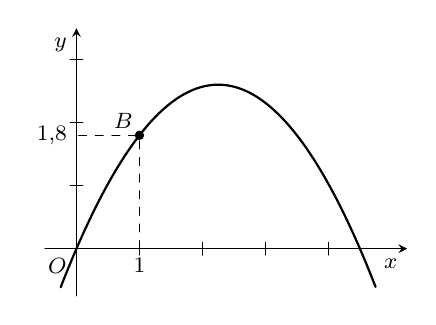
\begin{tikzpicture}[scale=0.8, font=\footnotesize, line join=round, line cap=round, >=stealth,cham/.style={circle,fill,inner sep=1.2pt}]
				\def\hso{-18/35*\x*\x+81/35*\x}
				\draw[thick,samples=200,smooth]plot[domain=-.25:4.75](\x,{\hso});
				\draw[->](-.5,0)--(5.25,0)node[below left]{$x$};
				\draw[->](0,-.75)--(0,3.5)node[below left]{$y$};
				\foreach \i in {1,...,4}{\draw (\i,.1)--(\i,-.1);}
				\foreach \i in {1,...,3}{\draw (.1,\i)--(-.1,\i);}
				\path (0,0) node[below left]{$O$};
				\draw[dashed,very thin] (1,0)node[below]{$1$}|-
				node[cham]{}node[above left=-1pt]{$B$}(0,1.8)node[left]{$1{,}8$};
			\end{tikzpicture}
		}
		Thay toạ độ các điểm trên vào hàm số, ta được $c=0$ và hệ phương trình: $\heva{&4,5^{2} a + 4{,}5b = 0 \\& 1^{2} a+1 b=1{,}8} \Leftrightarrow \heva{&a=\dfrac{-18}{35} \\& b=\dfrac{81}{35},}$\\
		Suy ra ta có hàm số: $y=\dfrac{-18}{35} x^2+\dfrac{81}{35} x$.\\
		Khi đó, ta có hoành độ đỉnh của đồ thị là $ x=-\dfrac{b}{2a}=\dfrac{9}{4} $.\\
		Từ đó, đỉnh của đồ thị hàm số trên có tung độ là $\dfrac{-18}{35} \cdot\left(\dfrac{9}{4}\right)^{2}+\dfrac{81}{35} \cdot \dfrac{9}{4} \approx 2,6$.\\
		Vậy chiều cao của cổng là khoảng $2{,}6$ m.
	}
\end{vd}
\begin{vd}%[0D3V2-6]%[Dự án đề cương 2025]%[Đoàn Minh Tâm]
	Một rạp chiếu phim có sức chứa $1\ 000$ người. Với giá vé là $40\ 000$ đồng, trung bình sẽ có khoảng $300$ người đến rạp xem phim mỗi ngày. Để tăng số lượng vé bán ra, rạp chiếu phim đã khảo sát thị trường và thấy rằng nếu giá vé cứ giảm $10\ 000$ đồng thì sẽ có thêm $100$ người đến rạp mỗi ngày.
	\begin{enumerate}
		\item Tìm công thức của hàm số $R(x)$ mô tả doanh thu từ tiền bán vé mỗi ngày của rạp chiếu phim khi giá vé là $x$ nghìn đồng.
		\item Tìm mức giá vé để doanh thu từ tiền bán vé mỗi ngày của rạp là lớn nhất.
	\end{enumerate}
	\loigiai{
		\begin{enumerate}
			\item Khi giá vé là $x$ (nghìn đồng) thì số tiền giảm giá mỗi vé so với mức giá cũ là $40-x$ (nghìn đồng).\\
			Số người tăng lên sau khi giảm giá vé là $\dfrac{100(40-x)}{10}=10(40-x)$.\\
			Số người đến rạp chiếu phim mỗi ngày sau khi giảm giá là
			$$300+10(40-x)=700-10x.$$
			Công thức của hàm số $R(x)$ mô tả doanh thu từ tiền bán vé mỗi ngày khi giá vé là $x$ (nghìn đồng) là
			$$R(x)=x(700-10x)=-10x^2+700x \text{ (nghìn đồng).}$$
			\item Hàm số $R(x)=-10x^2+700x$ là hàm số bậc hai có $ a=-10 <0 $ nên bề lõm hướng xuống dưới.\\
			Đồ thị hàm số có đỉnh là $ \heva{&x_I=-\dfrac{700}{2\cdot (-10)}=35\\&y_I=-10\cdot35^2+700\cdot 35=12\,250.} $\\
			Ta có bảng biến thiên như sau
			\begin{center}
				
\begin{tikzpicture}[>=stealth]
					\tkzTabInit[nocadre=false,lgt=1,espcl=2,deltacl=0.5]{$x$/.7,$R(x)$/2}
					{$-\infty$ , $35$ , $+\infty$}
					\tkzTabVar{-/$-\infty$ , +/$12\,250$ , -/$-\infty$}
				\end{tikzpicture}
			\end{center}
			 Do đó hàm số đạt giá trị lớn nhất tại $x-35$ và $R(35)=12\ 250$.\\
			Vậy doanh thu lớn nhất mà rạp chiếu có thể thu được mỗi ngày là $12\ 250\ 000$ đồng khi giá bán mỗi vé là $35\ 000$ đồng.
		\end{enumerate}
	}%<MyLT2>
\end{vd}


%-----------------------------------------------------------------------------
\subsection{Bài tập rèn luyện}
\ind{PHẦN I.} \inden{Câu trắc nghiệm nhiều phương án lựa chọn. Mỗi câu hỏi học sinh chỉ chọn một phương án.}\\
\setcounter{ex}{0}
\Opensolutionfile{ans}[ans/0D3-Bai2-TN]%--Đặt tên 2D1-Bai1-Dang1-TN
\begin{ex}[\textit{Trích đề thi HKI - Trường Nguyễn Công Trứ - Năm học 2024-2025}]%[0D3N2-1]%[Dự án đề cương 2025]%[Đoàn Minh Tâm]
	Với giá trị nào của tham số $m$ thì hàm số $y=(m+1)x^4-2x^2+2023$ là hàm số bậc hai?
	\choice
	{$m=0$}
	{$m=2$}
	{$m=1$}
	{\True $m=-1$}
	\loigiai{
		Hàm số  $y=(m+1)x^4-2x^2+2023$ là hàm số bậc hai $\Leftrightarrow m+1=0\Leftrightarrow m=-1$.
	}
\end{ex}

\begin{ex}[\textit{Trích đề thi HKI - Trường Lê Thánh Tôn - Năm học 2023-2024}]%[0D3N2-3]%[Dự án đề cương 2025]%[Đoàn Minh Tâm]
	Hàm số bậc hai $y=ax^2+bx+c$ có bảng biến thiên sau đây. Hãy tìm tọa độ đỉnh $S$ của đồ thị hàm số đã cho.
	\begin{center}
		
\begin{tikzpicture}
			\tkzTabInit[lgt=1.2,espcl=3]
			{$x$/0.7,$y$/2}
			{$-\infty$,$2$,$+\infty$}
			\tkzTabVar{+/$+\infty$,-/$-5$,+/$+\infty$}
		\end{tikzpicture}
	\end{center}
	\choice
	{$S(5;-2)$}
	{\True $S(2;-5)$}
	{$S(-2;5)$}
	{$S(-5;2)$}
	\loigiai{
		Tọa độ đỉnh của đồ thị hàm số là $S(2;-5)$.
	}
\end{ex}

\begin{ex}[\textit{Trích đề thi HKI - Trường Tân Túc - Năm học 2023-2024}]%[0D3N2-1]%[Dự án đề cương 2025]%[Đoàn Minh Tâm]
	Tìm tọa độ đỉnh $S$ của parabol $y=x^2-2x+1$.
	\choice
	{$S(0; 1)$}
	{$S(0; 0)$}
	{$S(1; 1)$}
	{\True $S(1; 0)$}
	\loigiai{
		Parabol có hoành độ đỉnh là $x=-\dfrac{b}{2a}=-\dfrac{-2}{2\cdot1}=1$. Suy ra tung độ đỉnh $y=0$.\\
		Do đó tọa độ đỉnh $S(1;0)$.
	}
\end{ex}

\begin{ex}[\textit{Trích đề thi HKI - Trường Bùi Thị Xuân - Năm học 2023-2024}]%[0D3N2-1]%[Dự án đề cương 2025]%[Đoàn Minh Tâm]%
	Cho Parabol $(P)\colon y=x^2+3x+2$. Phương trình trục đối xứng của $(P)$ là
	\choice
	{$x=-3$}
	{$y=-\dfrac{3}{2}$}
	{\True $x=-\dfrac{3}{2}$}
	{$y=-3$}
	\loigiai
	{
		Trục đối xứng của $(P)$ là $x=-\dfrac{b}{2a}=-\dfrac{3}{2}$.
	}
\end{ex}

\begin{ex}[\textit{Trích đề thi HKI - Trường Nguyễn Thái Bình - Năm học 2024-2025}]%[0D3N2-1]%[Dự án đề cương 2025]%[Đoàn Minh Tâm]
	Cho $(P) \colon y=x^2+bx+1$ đi qua điểm $A(-1;3)$. Khi đó
	\choice
	{\True $b=-1$}
	{$b=3$}
	{$b=1$}
	{$b=-2$}
	\loigiai{
		Vì $(P)$ đi qua $A(-1;3)$ nên ta có $3=(-1)^2-b+1 \Leftrightarrow b=-1$.
	}
\end{ex}

\begin{ex}[\textit{Trích đề thi HKI - Trường Hồ Thị Bi - Năm học 2023-2024}]%[0D3N2-1]%[Dự án đề cương 2025]%[Đoàn Minh Tâm]
	Cho hàm số $y=ax^2+bx+c$ có bảng biến thiên như sau
	\begin{center}
		
\begin{tikzpicture}
			\tkzTabInit
			[lgt=1.5,espcl=4] % tùy chọn
			{$x$/1, $y$/2.5} % cột đầu tiên
			{$-\infty$, $2$, $+\infty$} % hàng 1 cột 2
			\tkzTabVar{+/ $+\infty$, -/ $3$ , +/ $+\infty$} % hàng 3 cột 2
		\end{tikzpicture}
	\end{center}
	Khẳng định nào sau đây là đúng?
	\choice
	{$a\le 0$}
	{$a\ge 0$}
	{\True $a> 0$}
	{ $a<0$}
	\loigiai{
		Dựa vào bảng biến thiên, ta thấy $a>0$.
	}
\end{ex}

\begin{ex}[\textit{Trích đề thi HKI - Trường Tân Túc - Năm học 2023-2024}]%[0D3N2-2]%[Dự án đề cương 2025]%[Đoàn Minh Tâm]
	\immini{
		Hàm số nào sau đây có bảng biến thiên như hình vẽ?
		\choice
		{$y=-x^2+2 x-3$}
		{$y=x^2-2 x+3$}
		{\True $y=-x^2+2 x+1$}
		{$y=x+1$}
	}
	{
		
\begin{tikzpicture}
			\tkzTabInit[lgt=1.2,espcl=2, nocadre] % tùy chọn
			{$x$/.8, $y$/2} % cột đầu tiên
			{$-\infty$, $1$, $+\infty$}
			\tkzTabVar{-/$-\infty$,+/ $2$,-/$-\infty$}
		\end{tikzpicture}
	}
	\loigiai{
		Hàm số trong bảng biến thiên là hàm số bậc hai, có hệ số $a<0$, tọa độ đỉnh $I(1;2)$.\\
		Do đó hàm số $y=-x^2+2 x+1$ thỏa mãn.
	}
\end{ex}

\begin{ex}[\textit{Trích đề thi HKI - Trường Bùi Thị Xuân - Năm học 2023-2024}]%[0D3N2-2]%[Dự án đề cương 2025]%[Đoàn Minh Tâm]
	Cho parabol $(P)\colon y=-x^2+4 x+5$. Phát biểu nào sau đây đúng?
	\choice
	{Giá trị lớn nhất của hàm số bằng $2$}
	{\True Giá trị lớn nhất của hàm số bằng $9$}
	{Giá trị nhỏ nhất của hàm số bằng $9$}
	{Giá trị nhỏ nhất của hàm số bằng $2$}
	\loigiai
	{
		Ta có đỉnh Parabol là $I\left(2;9\right)$, $a=-1<0$ suy ra giá trị lớn nhất là $\max y=9$.
	}
\end{ex}

\begin{ex}[\textit{Trích đề thi HKI - Trường Bùi Thị Xuân - Năm học 2023-2024}]%[0D3N2-4]%[Dự án đề cương 2025]%[Đoàn Minh Tâm]
	Biết parabol $\left(P\right)\colon y=x^2+3x+c$ cắt trục hoành tại điểm có hoành độ bằng $-5$. Tìm $c$.
	\choice
	{$c=10$}
	{$c=-5$}
	{\True $c=-10$}
	{$c=15$}
	\loigiai{
		Theo giả thiết, ta có parabol $\left(P\right)\colon y=x^2+3x+c$ cắt trục hoành tại điểm $A\left(-5;0\right)$ nên ta được
		$$ (-5)^2+3\cdot (-5)+c=0 \Leftrightarrow c=-10.$$
	}
\end{ex}

\begin{ex}[\textit{Trích đề thi HKI - Trường THTH Sài Gòn - Năm học 2023-2024}]%[0D3N2-4]%[Dự án đề cương 2025]%[Đoàn Minh Tâm]
	Đồ thị của hàm số $y=x^2-3x+1$ cắt trục tung tại điểm có tọa độ là
	\choice
	{$\left(1;0\right)$}
	{$\left(0;-1\right)$}
	{\True $\left(0;1\right)$}
	{$\left(-1;0\right)$}
	\loigiai{
		Ta có $x=0$ thay vào ta được $y=1$.
	}
\end{ex}

\begin{ex}[\textit{Trích đề thi HKI - Trường Mạc Đĩnh Chi - Năm học 2024-2025}]%[0D3H2-3]%[Dự án đề cương 2025]%[Đoàn Minh Tâm]
	Đỉnh của parabol $(P)\colon y=2x^2-4x+6$ thuộc đường thẳng nào sau đây?
	\choice
	{$\Delta_1\colon y=x+4$}
	{$\Delta_2\colon y=2x+3$}
	{\True $\Delta_3\colon y=3x+1$}
	{$\Delta_4\colon y=4x-5$}
	\loigiai{
		Gọi $ I $ là đỉnh của parabol, khi đó hoành độ đỉnh là $ x=-\dfrac{-4}{2\cdot 2}=1 $.\\
		Tung độ đỉnh là $ y=2\cdot 1^2-4\cdot 1+6=4 $.\\
		Nên đỉnh có tọa độ là $ I(1;4) $ và tọa độ này thỏa mãn phương trình của $ \Delta_3 \colon y=3x+1$ (vì $ 4= 3\cdot 1+1 $).
	}
\end{ex}

\begin{ex}[\textit{Trích đề thi HKI - Trường Lê Quý Đôn - Năm học 2023-2024}]%[0D3H2-3]%[Dự án đề cương 2025]%[Đoàn Minh Tâm]
	\immini
	{
		Cho parabol $(P)\colon y=ax^2+bx+c$ có đồ thị như hình vẽ. Chọn đáp án đúng.
		\choice
		{\True $a>0$, $b<0$, $c>0$}
		{$a<0$, $b>0$, $c<0$}
		{$a>0$, $b>0$, $c<0$}
		{$a>0$, $b>0$, $c>0$}
	}
	{
		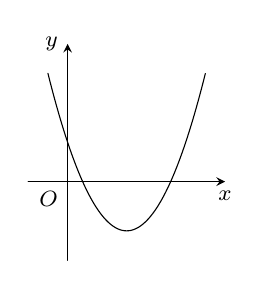
\begin{tikzpicture}[scale=0.5, font=\footnotesize, line join=round, line cap=round, >=stealth]
			\draw[->](-1,0)--(4,0)node[below]{$x$};
			\draw[->](0,-2)--(0,3.5)node[left]{$y$};
			\draw[smooth, samples=100, domain=-0.5:3.5]plot(\x,{(\x)^2-3*(\x)+1});
			\path(0,0)node[below left]{$O$};
		\end{tikzpicture}
	}
	\loigiai
	{
		Từ đồ thị, ta có
		\begin{itemize}
			\item $a>0$ vì đồ thị hàm số có bề lõm hướng lên.
			\item Giao điểm của $(P)$ với trục $Oy$ nằm phía trên trục $Ox$ nên $c>0$.
			\item Hoành độ đỉnh $-\dfrac{b}{2a}>0 \Leftrightarrow b<0$ (vì $a>0$).
		\end{itemize}
		Vậy $a>0$, $b<0$, $c>0$.
	}
\end{ex}

\begin{ex}[\textit{Trích đề thi HKI - Trường Chuyên Lê Quý Đôn - Ninh Thuận - Năm học 2024-2025}]%[0D3H2-2]%[Dự án đề cương 2025]%[Đoàn Minh Tâm]
	Cho hàm bậc hai $y=ax^{2}+bx+c$ $(a\ne0)$ có bảng biến thiên như hình vẽ bên dưới.
	\begin{center}
		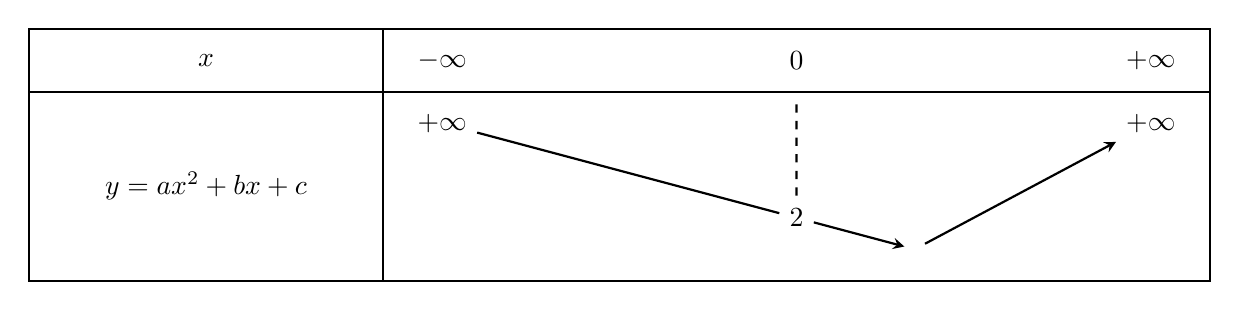
\begin{tikzpicture}[yscale=.8,xscale=1.5,thick,>=stealth]
			\begin{scope}[shift={(-.5,.5)}]
				\draw
				(-2,0) rectangle +(10,-4)
				(-2,-1)--+(0:10)
				(1,0)--+(-90:4)
				;
			\end{scope}
			\path
			(-1,0) node{$x$} % <<< dòng 1
			++(0:2) node{$-\infty$}
			++(0:3) node(A){$0$}
			++(0:3) node{$+\infty$}
			(-1,-2) node{$y=ax^2+bx+c$}       % <<< dòng 2
			(1,-1) node (H) {$+\infty$}
			++(0:3)++(-90:1.5) node (I) {$2$}
			++(0:1)++(-90:0.5) node (J) {}
			++(0:2)++(90:2) node (K) {$+\infty$}
			;
			\draw[->] (H)--(I)--(J);
			\draw[->] (J)--(K);
			\draw[dashed] (A)+(-90:0.7) -- (I);
		\end{tikzpicture}
	\end{center}
	Khi đó, dấu của các hệ số $a$, $b$, $c$ là
	\choice
	{\True $a>0$, $b<0$, $c>0$}
	{$a>0$, $b>0,$ $c>0$}
	{$a>0$, $b<0$, $c<0$}
	{$a>0$, $b>0$, $c<0$}
	\loigiai{Ta có bề lõm của parabol hướng lên nên $a>0$.\\
		Với $x=0$, ta được $y=2$ nên $2=c$ do đó $c>0$.\\
		Từ bảng biến thiên, ta có hoành độ đỉnh dương nên $-\dfrac{b}{2a}>0$ mà $a>0$ nên ta được $b<0$.\\
		Vậy $a>0$, $b<0$, $c>0$
	}
\end{ex}

\begin{ex}[\textit{Trích đề thi HKI - Trường Bùi Thị Xuân - Năm học 2023-2024}]%[0D3H2-3]%[Dự án đề cương 2025]%[Đoàn Minh Tâm]
	Hình sau đây là đồ thị hàm số nào?
	\begin{center}
		\begin{tikzpicture}[scale=0.8]
			\def\xmin{-2} \def\xmax{4}
			\def\ymin{-1} \def\ymax{4}
			\def\f(#1){(#1)^2-3*(#1)+2}
			\foreach \x in {1,2} \draw (\x,2pt)--(\x,-2pt) node [below] {$\x$};
			\draw[-stealth] (\xmin,0)--(\xmax,0)node[below]{$x$};
			\foreach \y in {2} \draw (2pt,\y)--(-2pt,\y) node [left] {$\y$};
			\draw[-stealth] (0,\ymin)--(0,\ymax)node[right]{$y$};
			\filldraw (0,0)node[above left]{$O$} circle (1.5pt);
			\clip (\xmin,\ymin) rectangle (\xmax,\ymax);
			\draw[samples=100,domain=\xmin:\xmax,smooth,red] plot (\x,{\f(\x)});
		\end{tikzpicture}
	\end{center}
	\choice
	{$y=-x^2-x+2$}
	{\True $y=x^2-3x+2$}
	{$y=x^2-x+1$}
	{$y=-x^2+x+1$}
	\loigiai
	{
		Gọi $(P)\colon y=ax^2+bx+c$ $\left(a\ne 0\right)$.\\
		Đồ thị hàm số cắt trục hoành tại $x=1$ và $x=2$ suy ra $y=f(x)=a\left(x-1\right)\left(x-2\right) \quad (1)$.\\
		$(P)$ cắt trục tung tại $\left(0;2\right)$ nên ta thay $x=0$, $y=2$ vào phương trình $(1)$ suy ra $a=1$.\\
		Vậy phương trình $(P)\colon y=\left(x-1\right)\left(x-2\right)=x^2-3x+2$.
	}
\end{ex}

\begin{ex}[\textit{Trích đề thi HKI - Trường Bùi Thị Xuân - Năm học 2023-2024}]%[0D3H2-1]%[Dự án đề cương 2025]%[Đoàn Minh Tâm]
	Cho parabol $(P)\colon y=ax^2+b x-4$ và trục đối xứng $x=-2$ và đi qua điểm $A\left(1;6\right)$. Tính $b-a$.
	\choice
	{$b-a=-10$}
	{$b-a=-6$}
	{\True $b-a=6$}
	{$b-a=10$}
	\loigiai
	{
		Trục đối xứng $x=-2\Rightarrow-\dfrac{b}{2a}=-2\Leftrightarrow 4a-b=0$.\\
		$(P)$ đi qua điểm $A(1;6)$ nên thay $x=1$, $y=6$ vào phương trình $(P)$ suy ra \[a+b-4=6\Leftrightarrow a+b=10.\]
		Vậy ta có hệ phương trình $\heva{& 4a-b=0 \\ & a+b=10}\Leftrightarrow\heva{& a=2 \\ & b=8.}$\\
		Vậy $b-a=8-2=6$.
	}
\end{ex}

\begin{ex}[\textit{Trích đề thi HKI -Trường Nguyễn Khuyến - Năm học 2023-2024}]%[0D3H2-1]%[Dự án đề cương 2025]%[Đoàn Minh Tâm]%
	Cho hàm số $y=a x^2+b x+c$ $(a \neq 0)$. Biết rằng đồ thị hàm số có đỉnh $I(2 ;-7)$ và đi qua điểm $M(-1 ; 2)$. Giá trị của biểu thức $S=a+b-c$ bằng
	\choice
	{$S=-6$}
	{\True $S=0$}
	{$S=2$}
	{$S=-7$}
\loigiai{
	Do hàm số có đỉnh là $I(2;-7)$ và qua điểm $M(-1;2)$ nên ta có hệ sau\\
	$$\heva{&-\dfrac{b}{2a}=2\\&-7=2^2a+2b+c\\&2=(-1)^2a+(-1)b+c}\Leftrightarrow \heva{&4a+b=0\\&4a+2b+c=-7\\&a-b+c=2}\Leftrightarrow \heva{&a=1\\&b=-4\\&c=-3.}$$
	Vậy $S=1+(-4)-(-3)=0$.
}
\end{ex}

\begin{ex}%[Dự án đề cương 2025]%[Đoàn Minh Tâm]%[0D3H2-2]
		Hàm số nào sau đây đồng biến trên khoảng $(2;+\infty)$?
		\choice
		{$y=-x+4$}
		{\True $y=2x^2-8x$}
		{$y=x^2-6x+5$}
		{$y=-x^2+4x+3$}
		\loigiai{
			Xét hàm số $y=2x^2-8x$.\\
			Tọa độ đỉnh $I(2;-8)$.\\
			Bảng biến thiên
			\begin{center}
				
\begin{tikzpicture}
					\tkzTabInit[nocadre=false,lgt=1.2,espcl=2.5,deltacl=0.6]
					{$x$ /0.8,$y$ /2}
					{$-\infty$,$2$,$+\infty$}
					\tkzTabVar{+/$+\infty$,-/$-8$,+/$+\infty$}
				\end{tikzpicture}
			\end{center}
			Hàm số đã cho đồng biến trên $(2;+\infty)$ và nghịch biến trên $(-\infty;2)$.
		}
\end{ex}

\begin{ex}[\textit{Trích đề thi HKI - Trường Bùi Thị Xuân - Năm học 2023-2024}]%[0D3H2-6]%[Dự án đề cương 2025]%[Đoàn Minh Tâm]
	Một cổng chào có hình parabol như hình vẽ dưới đây, biết khoảng cách giữa hai chân cổng bằng $20$ m và điểm $M$ trên cổng có tọa độ $(2;6)$. Chiều cao $h$ của cổng gần nhất với kết quả nào sau đây?
	\begin{center}
		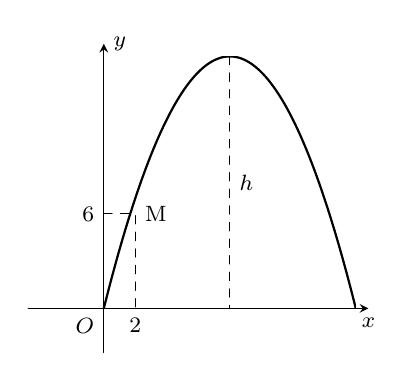
\begin{tikzpicture}[scale=0.8, font=\footnotesize, line join=round, line cap=round, >=stealth]
			\def\xmin{-1}\def\xmax{4}\def\ymin{-0.5}\def\ymax{4}
			%\def\c{$2-\sqrt{3}$}
			\draw[->] (\xmin-0.2,0)--(\xmax+0.2,0) node[below] {\footnotesize $x$};
			\draw[->] (0,\ymin-0.2)--(0,\ymax+0.2) node[right] {\footnotesize $y$};
			\draw (0,0) node [below left] {\footnotesize $O$};
			\foreach \x in {}\draw (\x,0.1)--(\x,-0.1) node [below] {\footnotesize $\x$};
			\foreach \y in {}\draw (0.1,\y)--(-0.1,\y) node [left] {\footnotesize $\y$};
			\clip (\xmin,\ymin) rectangle (\xmax,\ymax);
			\draw[thick,smooth,samples=200,domain=0:\xmax] plot (\x,{-1*((\x)^2)+4*\x});
			\draw [dashed] (2,4)--(2,2) node [right]{$h$}--(2,0);
			\draw [dashed] (0,1.5) node [left]{$6$}--(0.5,1.5) node [right]{M}--(0.5,0) node [below]{$2$};
		\end{tikzpicture}
	\end{center}
	\choice
	{$h=20$ m}
	{$h=15{,}7$ m}
	{\True $h=16{,}7$ m}
	{$h=10$ m}
	\loigiai{
		\immini{
			Giả sử parabol $(P): y=ax^2+bx+c \,(a\neq0)$.\\
			Do đồ thị hàm số cắt trục $Ox$ tại hai điểm $O(0; 0)$ và $A(20,0)$ nên ta có $\heva{&c=0\\&20^2a+20b=0.}$\\
			Lại có đồ thị hàm số đi qua $M(2;6)$ nên ta có $2^2a+2b=6$.\\
			Ta có hệ phương trình \[\heva{&20^2a+20b=0\\&2^2a+2b=6}\Leftrightarrow\heva{&a=-\dfrac{1}{6}\\&b=\dfrac{10}{3}.}\]
			Do đó $(P)\colon y=-\dfrac{1}{6}x^2+\dfrac{10}{3}x$.\\
			Parabol $(P)$ có đỉnh $I\left(10;\dfrac{50}{3}\right)$. Khi đó $h=y_I=\dfrac{50}{3}\approx 16{,}7$ (m).
		}{
			\begin{tikzpicture}[scale=0.8, font=\footnotesize, line join=round, line cap=round, >=stealth]
				\def\xmin{-1}\def\xmax{4.5}\def\ymin{-0.5}\def\ymax{5}
				%\def\c{$2-\sqrt{3}$}
				\draw[->] (\xmin-0.2,0)--(\xmax+0.2,0) node[below] {\footnotesize $x$};
				\draw[->] (0,\ymin-0.2)--(0,\ymax+0.2) node[right] {\footnotesize $y$};
				\draw (0,0) node [below left] {\footnotesize $O$};
				\foreach \x in {}\draw (\x,0.1)--(\x,-0.1) node [below] {\footnotesize $\x$};
				\foreach \y in {}\draw (0.1,\y)--(-0.1,\y) node [left] {\footnotesize $\y$};
				\clip (\xmin,\ymin) rectangle (\xmax,\ymax);
				\draw[thick,smooth,samples=200,domain=\xmin:\xmax] plot (\x,{-1*((\x)^2)+4*\x});
				\draw [dashed] (0,4) node[left]{$\dfrac{50}{3}$}--(2,4) node [above]{$I$}--(2,2) node [right]{$h$}--(2,0) node [below]{$10$} (4,0) node [above right]{$A$} (4,0) node [below left]{$20$};
				\draw [dashed] (0,1.5) node [left]{$6$}--(0.5,1.5) node [right]{M}--(0.5,0) node [below]{$2$};
			\end{tikzpicture}
		}
	}
\end{ex}

\begin{ex}[\textit{Trích đề thi HKI - Trường Mạc Đĩnh Chi - Năm học 2024-2025}]%[0D3V2-6]%[Dự án đề cương 2025]%[Đoàn Minh Tâm]
	Một cửa hàng bán balo tiến hành khảo sát thị trường và thấy rằng, nếu giá bán mỗi chiếc balo là $x$ (nghìn đồng) thì số lượng balo bán được mỗi ngày là $\left(200-x\right)$ chiếc. Tính lợi nhuận cao nhất mà cửa hàng có thể thu được trong mỗi ngày biết rằng mỗi chiếc balo cửa hàng nhập về có giá $60$ nghìn đồng.
	\choice
	{$5\,100\,000$ đồng}
	{$5\,000\,000$ đồng}
	{$4\,800\,000$ đồng}
	{\True $4\,900\,000$ đồng}
	\loigiai{
		Từ dữ kiện đề bài, ta có $ 0<x<200 $.\\
		Vậy lợi nhuận thu được được biểu diễn theo hàm $ f(x)=x\left(200-x\right)-60(200-x)=-x^2+260x-12\,000$ (nghìn đồng).\\
		Ta có $ f(x) $ là hàm bậc hai có bảng biến thiên như sau
		\begin{center}
			
\begin{tikzpicture}[>=stealth]
				\tkzTabInit[nocadre=false,lgt=1,espcl=2,deltacl=0.5]{$x$/.7 ,$y$/2}
				{$0$ , $130$ , $200$}
				\tkzTabVar{-/$-\infty$ , +/$4\,900$ , -/$-\infty$}
			\end{tikzpicture}
		\end{center}
		Dựa vào bảng biến thiên, số tiền lợi nhuận lớn nhất là $ 4\,900\,000 $ đồng.
	}
\end{ex}


\begin{ex}%[0D3V2-6]%[Dự án đề cương 2025]%[Đoàn Minh Tâm]
	Một doanh nghiệp tư nhân A chuyên kinh doanh xe gắn máy các loại. Hiện nay doanh nghiệp đang tập trung chiến lược vào kinh doanh xe Honda Future Fi với chi phí mua vào một chiếc là $27$ (triệu đồng) và bán ra với giá là $31$ triệu đồng. Với giá bán này thì số lượng xe mà khách hàng sẽ mua trong một năm là $600$ chiếc. Nhằm mục tiêu đẩy mạnh hơn nữa lượng tiêu thụ dòng xe đang ăn khách này, doanh nghiệp dự định giảm giá bán và ước tính rằng nếu giảm $1$ triệu đồng mỗi chiếc xe thì số lượng xe bán ra trong một năm là sẽ tăng thêm $200$ chiếc. Vậy doanh nghiệp phải định giá bán mới là bao nhiêu để sau khi đã thực hiện giảm giá, lợi nhuận thu được sẽ là cao nhất.
	\choice
	{$30$ triệu đồng}
	{$29$ triệu đồng}
	{\True $30{,}5$ triệu đồng}
	{$29{,}5$ triệu đồng}
	\loigiai{
		Gọi $x$ (triệu đồng) là số tiền mà doanh nghiệp A dự định giảm giá $\left( 0\le x\le 4 \right)$.\\
		Khi đó lợi nhuận thu được khi bán một chiếc xe là $31-x-27=4-x$ (triệu đồng).\\
		Số xe mà doanh nghiệp sẽ bán được trong một năm là $600+200x$ (chiếc).\\
		Lợi nhuận mà doanh nghiệp thu được trong một năm là
		$$f\left( x \right)=\left( 4-x \right)\left( 600+200x \right)=-200x^2+200x+2400.$$
		Xét hàm số $f\left( x \right)=-200x^2+200x+2400$ trên đoạn $\left[0;4 \right]$ có bảng biến thiên
		\begin{center}
			
\begin{tikzpicture}
				\tkzTabInit[nocadre=false,lgt=1.2,espcl=2.5,deltacl=0.6]
				{$x$ /1,$y$ /2}
				{$0$,$\dfrac{1}{2}$,$4$}
				\tkzTabVar{-/$2400$, +/$2450$,-/$0$}
			\end{tikzpicture}
		\end{center}
		Vậy $\underset{\left[0;4 \right]}{\mathop{\max}}f\left( x \right)=2450\Leftrightarrow x=\dfrac{1}{2}$.\\
		Vậy giá mới của chiếc xe là $31-0{,}5=30{,}5$ triệu đồng thì lợi nhuận thu được là cao nhất.}%<MyLT2>
\end{ex}
\Closesolutionfile{ans}

\ind{PHẦN II.} \inden{Câu trắc nghiệm đúng sai. Trong mỗi ý a), b), c), d) ở mỗi câu, học sinh chọn đúng hoặc sai.}\\
\Opensolutionfile{ans}[ans/0D3-Bai2-DS]%--Đặt tên 2D1-Bai1-Dang1-TN
\setcounter{ex}{0}


\begin{ex}%[0D3H2-3]%[Dự án đề cương 2025]%[Đoàn Minh Tâm]
	Cho hàm số bậc hai $y=x^2-2x-3$.
	\choiceTF
	{\True Đồ thị hàm số nhận đường thẳng $x=1$ làm trục đối xứng}
	{Hàm số trên đồng biến trên khoảng $(-\infty;1)$ và nghịch biến trên khoảng $(1;+\infty)$}
	{Hàm số trên đạt giá trị lớn nhất trên $\mathbb{R}$ là $-4$ khi $x=1$}
	{\True Đồ thị hàm số trên là Parabol có tọa độ đỉnh là $(1;-4)$}
	\loigiai{
		\begin{itemchoice}
			\itemch \textbf{Đúng}.\\
			Trục đối xứng $x=-\dfrac{b}{2a}=1$.
			\itemch \textbf{Sai}.\\
			Vì $a=1>0$ nên hàm số trên nghịch biến trên khoảng $(-\infty;1)$ và đồng biến trên khoảng $(1;+\infty)$.
			\itemch \textbf{Sai}.\\
			Do $a=1>0$ nên hàm số chỉ có giá trị nhỏ nhất chứ không có giá trị lớn nhất.
			\itemch \textbf{Đúng}.\\
			Hoành độ đinh $x=-\dfrac{b}{2a}=1$.\\
			Tung độ đỉnh $y=f(1)=1-2-3=-4$.\\
			Do đó, đồ thị hàm số trên là Parabol có tọa độ đỉnh là $(1;-4)$.
		\end{itemchoice}
	}
\end{ex}

\begin{ex}%[0D3H2-3]%[Dự án đề cương 2025]%[Đoàn Minh Tâm]
	\immini{
	Cho hàm số $f(x)=ax^{2}+bx+c$ có đồ thị như hình vẽ.
	\choiceTF
	{$f(1)=1$}
	{\True $a>0$}
	{$a+b+c>1$}
	{\True $a-b=10$}}{
	\begin{tikzpicture}[scale=1, font=\footnotesize, line join=round, line cap=round, >=stealth]
		\def\xmax{4}
		\def\xmin{-1}
		\def\ymax{2}
		\def\ymin{-1.5}
		\draw[->] (\xmin,0)--(\xmax,0)node[below]{ $x$};
		\draw[->] (0,\ymin)--(0,\ymax)node[left]{ $y$};
		\draw[fill=black] (0,0) circle(1pt)node[below left]{$O$};
		\clip (\xmin,\ymin) rectangle (\xmax,\ymax);
		\draw[smooth,domain=\xmin:\xmax] plot (\x,{2*(\x)^2-8*\x+13/2});
		\draw[dashed] (1,0)--(1,.5);
		\draw[dashed] (3,0)|-(0,.5);
		\draw[fill=black] (0,.5) circle(1pt)node[left]{$\dfrac{1}{2}$};
		\draw[fill=black] (1.5,0) circle(1pt) node[below right]{$\dfrac{3}{2}$};
		\draw[fill=black] (1,.5) circle(1pt);
		\draw[fill=black] (3,.5) circle(1pt);
		\draw[fill=black] (1.5,-1) circle(1pt);
		\draw (3.6,1.5) node{$f(x)$};
		\draw[dashed] (1.5,0)|-(0,-1);
		\foreach \d/\g in {1/-90,3/-90}
		\fill (\d,0) circle(1pt) + (\g:.3) node[rectangle,fill=white,inner sep=1.2]{$\d$};
		\foreach \d/\g in {-1/180}
		\fill (0,\d) circle(1pt) + (\g:.3) node[rectangle,fill=white,inner sep=1.2]{$\d$};
	\end{tikzpicture}
}
	\loigiai{
		\begin{itemchoice}
			\itemch\textbf{Sai}.\\
			Dựa vào đồ thị ta thấy $f(1)=\dfrac{1}{2}$.
			\itemch\textbf{Đúng}.\\
			Từ đồ thị ta có $a>0$.
			\itemch\textbf{Sai}.\\
			Ta có $a+b+c=f(1)=\dfrac{1}{2}<1$.
			\itemch\textbf{Đúng}.\\
			Từ đồ thị ta có hệ phương trình:
			$\heva{&f(1)=\dfrac{1}{2}\\&f\left(\dfrac{3}{2}\right)=-1\\&f(3)=\dfrac{1}{2}}
			\Leftrightarrow
			\heva{&a+b+c=\dfrac{1}{2}\\&	\dfrac{9}{4}a+\dfrac{3}{2}b+c=-1\\&9a+3b+c=\dfrac{1}{2}}
			\Leftrightarrow
			\heva{&a=2\\&b=-8\\&c=\dfrac{13}{2}.}$\\
			Do đó $a-b=10$.
		\end{itemchoice}
	}
\end{ex}

\begin{ex}%[0D3H2-3]]%[Dự án đề cương 2025]%[Đoàn Minh Tâm]
	Cho hàm số $y=ax^2+6x+c$ có đồ thị là parabol $(P)$. Biết $(P)$ có đỉnh là điểm $I(-1;-4)$.
	\choiceTF
	{\True $a=3$}
	{$c=1$}
	{Hàm số đồng biến trên khoảng $(-\infty;-1)$}
	{Giá trị lớn nhất của hàm số bằng $-4$}
	\loigiai{
		Hoành độ đỉnh $x_I=\dfrac{-6}{2a} \Leftrightarrow \dfrac{-6}{2a}=-1 \Leftrightarrow a =3$.\\
		Đỉnh $I(-1;-4) \in (P) \Leftrightarrow a\cdot (-1)^2+6\cdot (-1)+c=-4 \Leftrightarrow a+c=2 \Leftrightarrow c=-1.$\\
		Suy ra $y=3x^2+6x-1$.\\
		Bảng biến thiên
		\begin{center}
			
\begin{tikzpicture}
				\tkzTabInit[nocadre=false,lgt=1.2,espcl=2,deltacl=0.6]
				{$x$/1,$y$/2}
				{$-\infty$,$-1$,$+\infty$}
				\tkzTabVar{+/$+\infty$,-/$-4$,+/$+\infty$}
			\end{tikzpicture}
		\end{center}
		\begin{itemchoice}
			\itemch \textbf{Đúng}.
			\itemch \textbf{Sai}.
			\itemch \textbf{Sai}. Hàm số nghịch biến trên $(-\infty;-1)$.
			\itemch \textbf{Sai}. Hàm số không có giá trị lớn nhất.
		\end{itemchoice}
	}
\end{ex}

\begin{ex}%[0D3H2-1]%[Dự án đề cương 2025]%[Đoàn Minh Tâm]
	Cho hàm số bậc hai $y=ax^2+bx+c$ biết đồ thị hàm số đi qua điểm $A(-1;8)$ và có đỉnh $I(2;-1)$. Khi đó:
	\choiceTF
	{\True $a-b+c=8$}
	{$b=4a$ và $4a+2b+c=-1$}
	{\True $y=x^2-4x+3$}
	{Giá trị nhỏ nhất của hàm số đã cho trên đoạn $[-3;0]$ bằng $-1$}
	\loigiai{
		\begin{itemchoice}
			\itemch \textbf{Đúng}. Thay tọa độ điểm $A(-1;8)$ vào hàm số ta được $a-b+c=8$.
			\itemch \textbf{Sai}. $-\dfrac{b}{2a}=2\Rightarrow b=-4a$ và điểm $I(2;-1)$ thuộc đồ thị hàm số nên $4a+2b+c=-1$
			\itemch \textbf{Đúng}. Ta có hệ
			$\heva{&a-b+c=8\\&-\dfrac{b}{2a}=2\\&4a+2b+c=-1}\Leftrightarrow\heva{&a-b+c=8\\&4a+b=0\\&4a+2b+c=-1}\Leftrightarrow\heva{&a=1\\&b=-4\\&c=3.}$\\
			Do đó $y=x^2-4x+3$.
			\itemch \textbf{Sai}. Ta có bảng biến thiên của hàm số $y=x^2-4x+3$
			\begin{center}
				\begin{tikzpicture}[font=\normalsize,t style/.style={style=solid}]
					\tkzTabInit[nocadre=true, lgt=1.2, espcl=2.5, deltacl=0.5]
					{$x$/0.75, $y$/3}
					{$-\infty$, $-3$, $0$, $2$, $+\infty$}
					\path
					($(N11)!0.1!(N12)$) node (A1){$+\infty$}
					($(N41)!0.8!(N42)$) node (A2){$-1$}
					($(N51)!0.1!(N52)$) node (A3){$+\infty$}
					($(N21)!0.28!(N22)$) node[right]{$24$}
					($(N31)!0.61!(N32)$) node[left]{$3$}
					;
					\foreach \x/\y in {A1/A2, A2/A3}{
						\draw[-stealth] (\x)--(\y);
					}
					\draw (N21)--(N22) (N31)--(N32);
					\path [pattern=north east lines] (N21)--(N22)--(T12)--(T11)--cycle;
					\path [pattern=north west lines] (N31)--(N32)--(T22)--(T21)--cycle;
				\end{tikzpicture}
			\end{center}
			Từ đó ta suy ra giá trị nhỏ nhất của hàm số trên $[-3;0]$ bằng $3$.
		\end{itemchoice}
	}
\end{ex}


\begin{ex}%[0D3V2-6]%[Dự án đề cương 2025]%[Đoàn Minh Tâm]
	Một miếng nhôm có bề ngang $32$ cm được uốn cong tạo thành máng dẫn nước bằng cách chia tấm nhôm thành ba phần rồi gấp hai bên lại theo một góc vuông như hình vẽ dưới. Để đảm bảo kĩ thuật, diện tích mặt cắt ngang của máng dẫn nước phải lớn hơn hoặc bằng $120$ cm$^2$.\\
	\centerline
	{
		\begin{tikzpicture}[line cap=round,line join=round,font=\footnotesize,>=stealth]
			%\node[circle,shading=ball,minimum width=3cm] (ball) at (0,0) {};
			\path (0:0) coordinate(A) (0:4) coordinate(D) (60:3) coordinate(B) ($(B)+(D)-(A)$) coordinate(C) ($(A)!.3!(D)$) coordinate(E) ($(D)!.3!(A)$) coordinate(F) ($(B)!.3!(C)$) coordinate(H) ($(C)!.3!(B)$) coordinate(G);
			\fill[shading=ball,ball color=gray!30, minimum width=3cm] (A) -- (B) -- (C) --(D) -- cycle;
			\draw (A) -- (B) -- (C) -- (D) -- cycle (E)--(H) (F)--(G);
			\draw[<->] ([shift={(-90:.2)}]A) -- ([shift={(-90:.2)}]D) node[midway,below]{$32$ cm};
			\draw[<->] ([shift={(90:.1)}]B) -- ([shift={(90:.1)}]H) node[midway,above]{$x$ cm};
			\draw[<->] ([shift={(90:.1)}]G) -- ([shift={(90:.1)}]C) node[midway,above]{$x$ cm};
		\end{tikzpicture}
		\begin{tikzpicture}[line cap=round,line join=round,font=\footnotesize,>=stealth]
			\path (0:0) coordinate(A) (90:1) coordinate(B) ++(60:3) coordinate(C) ($(A)+(C)-(B)$) coordinate(D) (0:1.8) coordinate(E) ++(90:1) coordinate(H) ($(D)+(E)-(A)$) coordinate(F) ($(F)+(H)-(E)$) coordinate(G) ($(A)!.5!(D)$) coordinate(M) ++(90:1) coordinate(Q) ($(E)!.5!(F)$) coordinate(N) ++(90:1) coordinate(P);
			\fill[gray!30] (A) -- (B) --(C) -- (D) -- cycle;
			\fill[gray!60] (A) -- (D) --(F) -- (E) -- cycle;
			\fill[violet] (M) -- (N) --(P) -- (Q) -- cycle;
			\fill[green!40!black] (E) -- (F) -- (G) -- (H) -- cycle;
			\draw (A) -- (B) --(C) -- (D) -- cycle (E) -- (F) --(G) -- (H) -- cycle (A)--(E) (D)--(F);
			\draw[dashed] (M) -- (N) --(P) -- (Q) -- cycle;
			\draw[->] (E) ++(-10:1.5) node[below]{mặt cắt ngang} -- ([shift={(90:.4)}]$(M)!.5!(N)$);
			\draw[->] (C) ++(50:1.5) node[above]{chiều ngang mặt cắt} -- ([shift={(90:.05)}]$(P)!.5!(Q)$);
		\end{tikzpicture}
	}
	Xét tính đúng sai của các khẳng định dưới đây.
	\choiceTF
	{\True Chiều ngang mặt cắt ngang của máng dẫn nước là $(32-2x)\text{ cm}$}
	{Diện tích mặt cắt ngang của máng dẫn nước là $2x(32-2x) \text{ cm}^2$}
	{Với $x= 5 \text{ cm}$ thì máng dẫn nước đảm bảo kĩ thuật}
	{\True Diện tích mặt cắt ngang của máng dẫn nước lớn nhất bằng $128 \text{ cm}^2$}
	\loigiai
	{
		Gọi $S(x)$ là diện tích mặt cắt ngang của máng dẫn.\\
		Mặt cắt ngang là hình chữ nhật có chiều dọc là $x \text{ cm}$, chiều ngang là $(32-2x) \text{ cm}$. Khi đó $S(x) = x(32-2x) \text{ cm}^2$, với $0<x<16$.\\
		Với $x=5 \text{ cm}$ thì $S(5) = 5(32-2\cdot 5) = 110<120$ nên máng dẫn nước không đảm bảo kĩ thuật.\\
		Diện tích mặt ngang lớn nhất khi hàm số $S(x)$ đạt giá trị lớn nhất trên khoảng $(0;16)$.\\
		Ta có
		\[S(x) = x(32-2x) = -2x^2+32x = -2(x-8)^2+128\leq 128, \forall x\in (0;16).\]
		Đẳng thức $S(x)=128$ xảy ra khi $x=8$.\\
		Vậy diện tích mặt cắt ngang của máng dẫn nước lớn nhất bằng $128 \text{ cm}^2$.
		\begin{itemchoice}
			\itemch \textbf{Đúng}. Do chiều ngang mặt cắt ngang của máng dẫn nước là $(32-2x)\text{ cm}$.
			\itemch \textbf{Sai}. Do diện tích mặt cắt ngang của máng dẫn nước là $x(32-2x) \text{ cm}^2$
			\itemch \textbf{Sai}. Do $S(5) = 110<120$ nên máng dẫn nước không đảm bảo kĩ thuật.
			\itemch \textbf{Đúng}. Do diện tích mặt cắt ngang của máng dẫn nước lớn nhất bằng $128 \text{ cm}^2$.
		\end{itemchoice}
	}
\end{ex}

\Closesolutionfile{ans}

\ind{PHẦN III.} \inden{Câu trả lời ngắn.}\\
\setcounter{ex}{0}
\Opensolutionfile{ans}[ans/0D3-Bai2-TLN]%--Đặt tên 2D1-Bai1-DS


\begin{ex}%[0D3V2-4]%[Dự án đề cương 2025]%[Đoàn Minh Tâm]
	Cho hàm số $y = f(x) = x^2 + mx + n$ ($m, n \in \mathbb{R}$) có đồ thị là parabol ($P$). Tính $ P=2m+n $ của hàm số $f(x)$ biết rằng đồ thị ($P$) cắt trục hoành tại điểm $A$ có hoành độ bằng $3$ và có trục đối xứng là đường thẳng $x = \dfrac{5}{2}$.
	\shortans{$ -4 $}
	\loigiai{
		Ta có $x=\dfrac{-b}{2a}\Rightarrow\dfrac{5}{2}=\dfrac{-m}{2}\Rightarrow m=\dfrac{5\cdot 2}{-2}=-5$.\\
		Do ($P$) cắt trục hoành tại điểm $A$ có hoành độ bằng $3$ nên $A(3;0)\in (P) $.\\
		Suy ra $\Rightarrow 3m+n=-9\Rightarrow n=6$.\\
		Vậy $f(x)=x^2-5x+6$ nên $ P=2\cdot (-5)+6=-4$
	}
\end{ex}

\begin{ex}%[0D3V2-4]%[Dự án đề cương 2025]%[Đoàn Minh Tâm]
	Cho hàm số $y=ax^{2}+bx+c$ có đồ thị là parabol $(P)$. Biết rằng đường thẳng $y=-2$ cắt $(P)$ tại một điểm duy nhất, đường thẳng $y=2$ cắt $(P)$ tại hai điểm phân biệt có hoành độ lần lượt là $-1$ và $5$. Tính giá trị $T=a+2b+4c$.
	\par
	\shortans{$-4$}
	\loigiai{
		Vì $(P)$ có trục đối xứng là một đường thẳng song song hoặc trùng với $Oy$ và đường thẳng $y=2$ (vuông góc với trục đối xứng của $(P)$) cắt $(P)$ tại hai điểm phân biệt có hoành độ lần lượt là $-1$ và $5$, nên trục đối xứng của $(P)$ là đường thẳng $x=\dfrac{-1+5}{2}=2$.\\
		Vậy hoành độ của đỉnh $(P)$ là $x=2$ và điểm $A(-1;2)\in (P)$.\\
		Mà đường thẳng $y=-2$ cắt $(P)$ tại một điểm duy nhất nên đường thẳng $y=-2$ đi qua đỉnh của $(P)$.\\
		Vậy tung độ của đỉnh $(P)$ là $y=-2$.\\
		Suy ra tọa độ đỉnh của $(P)$ là $I(2;-2)$.\\
		Ta có $\heva{&-\dfrac{b}{2a}=2\\&a-b+c=2\\&4a+2b+c=-2}\Leftrightarrow\heva{&a=\dfrac{4}{9}\\&b=-\dfrac{16}{9}\\&c=-\dfrac{2}{9}.}$\\
		Vậy $T=a+2b+4c=-4$.\\
	}
\end{ex}

\begin{ex}%[0D3V2-6]%[Dự án đề cương 2025]%[Đoàn Minh Tâm]
	Khi một quả bóng được ném lên, nó sẽ đạt đến độ cao nào đó rồi rơi xuống. Biết quỹ đạo của quả bóng là một cung Parabol trong mặt phẳng với hệ tọa độ $Oth$, trong đó $t$ là thời gian (tính bằng giây), kể từ khi quả bóng được đá lên, $h$ là độ cao (tính bằng mét) của quả bóng. Giả thiết rằng quả bóng được đá lên từ độ cao $1{,}2$ m. Sau đó $1$ giây, nó đạt độ cao $8{,}5$ m và $2$ giây sau khi đá nó lên, nó ở độ cao $6$ m. Sau bao lâu thì quả bóng sẽ chạm đất kể từ khi đá lên (Tính chính xác đến hàng phần trăm)?
	\shortans{$2{,}58$}
	\loigiai{
		\immini{Do bóng được đá từ độ cao $1{,}2$ m nên trong hệ trục tọa độ $Oth$ ta có\\
			Parabol cắt trục $Oh$ tại điểm có tung độ $h=1{,}2$ m.\\
			Khi đó phương trình Parabol có dạng $h(t)=at^2+bt+1,2$, với $t > 0$.\\
			Theo giả thiết ta có hệ phương trình\\
			$\heva{&h(1)=a+b+1{,}2=8{,}5\\&h(2)=4a+2b+1{,}2=6}\Leftrightarrow\heva{&a+b=7{,}3\\&2a+b=2{,}4}\Leftrightarrow\heva{&a=-4{,}9\\&b=12{,}2.}$\\
			Do đó khi quả bóng chạm đất thì độ cao của quả bóng so với mặt đất bằng $0$.\\
			Vậy $0=-4{,}9t^2+12,2t+1{,}2\Rightarrow t\approx 2{,}58$.}{
			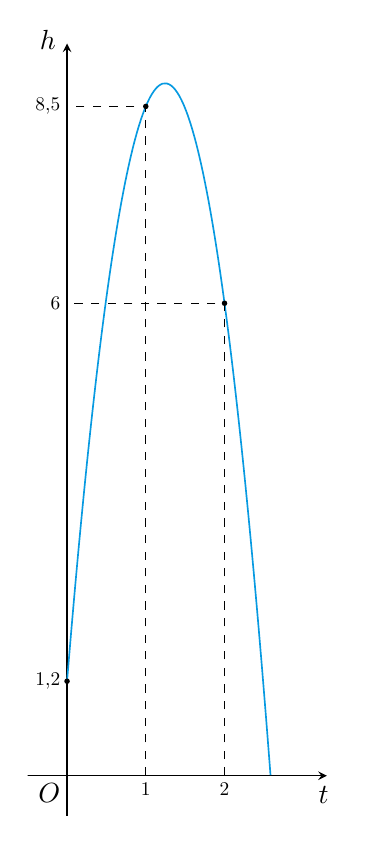
\begin{tikzpicture}[line cap=butt,line join=miter,>=stealth]
				\tikzset{declare function={xmin=-0.5-0.2;xmax=3+0.3;
						ymin=-0.5-0.2;ymax=9+0.3;
						f(\x)=- 49*(\x)^2/10 + 61*(\x)/5 + 6/5;},smooth,samples=50}
				\clip (-0.5,-0.5) rectangle (3.5,9.5);
				\draw[->] (xmin,0)--(xmax,0) node[shift={(-100:7pt)}]{$t$};
				\draw[->] (0,ymin)--(0,ymax) node[shift={(170:7pt)},font=\normalsize]{$h$};
				\fill (0,0) node[shift={(-135:9pt)}]{$O$};
				\begin{scope}
					\clip (xmin,ymin) rectangle (xmax,ymax);
					\draw[cyan!85!blue,semithick] plot[domain=0:2.584] (\x, {f(\x)});
					\fill (0,1.20) circle (1pt) node[left,,scale=.7]{$1{,}2$};
					\fill (1,8.5) circle (1pt);
					\fill (2,6) circle (1pt);
					\draw[dashed] (1,0)node[below,,scale=.7]{$1$}|-(0,8.5)node[left,scale=.7]{$8{,}5$} (2,0)node[below,,scale=.7]{$2$}|-(0,6)node[left,scale=.7]{$6$};
				\end{scope}

			\end{tikzpicture}}

	}
\end{ex}



\begin{ex}[\textit{Trích đề ôn tập GHKI - Trường Hồ Thị Bi - Năm học 2024-2025}]%[0D3V2-6]%[Dự án đề cương 2025]%[Đoàn Minh Tâm]
	Cầu Đông Trù là một cây cầu bắc qua sông Đuống, được xây dựng theo kiểu vòm ống thép, cầu gồm 3 nhịp chính trong đó 2 nhịp biên dài $80$ m và nhịp giữa sông dài $120$ m. Mỗi nhịp được kiến trúc bằng đường cong tựa như một parabol.
	Giả sử rằng mỗi nhịp của cầu là một parabol (như hình vẽ bên dưới). Một người đã dùng dây dọi (không giãn) gắn lên thành cầu ở vị trí $B$ và điều chỉnh độ dài dây dọi để quả nặng vừa chạm đất ở vị trí $H$ (khi lặng gió). Sau đó đo được chiều dài đoạn dây dọi $BH$ là $2{,}9$ m và khoảng cách từ chân trụ cầu đến quả nặng (đoạn $OH$) là $3$ m.
	Gọi khoảng cách từ đỉnh $S$ vòm đến mặt đường là $h$. Nếu dùng dữ liệu thu thập được và tính toán thì ước tính được độ cao $h$ là bao nhiêu? (Kết quả làm tròn đến hàng đơn vị).
	\begin{center}
		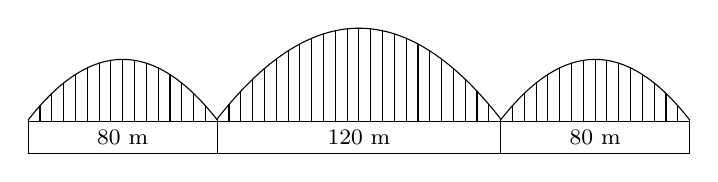
\begin{tikzpicture}[scale=.4, xscale=.75, font=\footnotesize, line join=round, line cap=round, >=stealth]
			\def\a{14}
			\pgfmathsetmacro\b{3*\a/7}
			\def\f(#1){-0.08*(#1)^2+2.97}
			\draw (-\a,0)--(\a,0) (-\a,-1)--(\a,-1);
			\foreach \i in {-\a,-\b,\b,\a} \draw (\i,0)--(\i,-1);
			\tikzset{cau/.pic={
					\draw[domain=-\b:\b, samples=100, scale=.4, xscale=.75]plot (\x, {\f(\x)});
			}}
			\tikzset{day1/.pic={
					\foreach \m in {-6,-5.5,...,6} \draw[scale=.4, xscale=.75] (\m,{\f(\m)})--(\m,0);
			}}
			\tikzset{day2/.pic={
					\foreach \m in {-6,-5.25,...,6} \draw[scale=.4, xscale=.75] (\m,{\f(\m)})--(\m,0);
			}}
			\draw (0,0) pic{cau} pic{day1};
			\draw (-10,0) pic[scale=2/3]{cau} pic[scale=2/3]{day2};
			\draw (10,0) pic[scale=2/3]{cau} pic[scale=2/3]{day2};
			\draw (0,-0.5) node{$120$ m} (-10,-0.5) node{$80$ m} (10,-0.5) node{$80$ m};
		\end{tikzpicture}
	\end{center}

	\begin{center}
		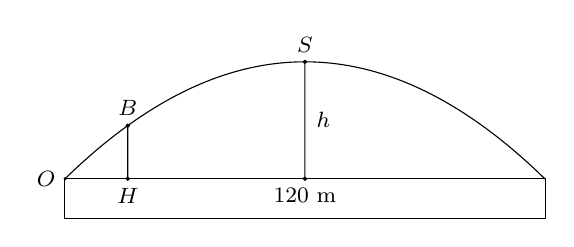
\begin{tikzpicture}[scale=.5, font=\footnotesize, line join=round, line cap=round, >=stealth]
			\def\a{14}
			\pgfmathsetmacro\b{3*\a/7}
			\def\f(#1){-0.08*(#1)^2+2.97}
			\tikzset{cau/.pic={
					\draw[domain=-\b-0.1:\b+0.1, samples=100, scale=.5]plot (\x, {\f(\x)});
			}}
			\draw (0,0) pic{cau};
			\draw (-\b-0.1,0)--(-\b-0.1,-1)--(\b+0.1,-1)--(\b+0.1,0)--cycle;
			\draw (-4.5,{\f(-4.5)}) node[above]{$B$}circle (1.2pt) -- (-4.5,0) node[below]{$H$} circle (1.2pt)
			(0,2.97) node[above]{$S$}circle (1.2pt)-- (0,0)circle (1.2pt);
			\fill[black] (-6.09,0) node[left]{$O$}circle (1.2pt) (0.05, 1.5) node[right]{$h$} (0,0)node[below]{$120$ m};
		\end{tikzpicture}

	\end{center}
	\shortans{$30$}
	\loigiai{

		\begin{center}
			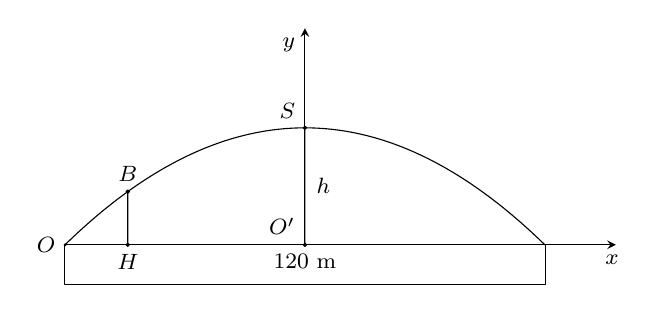
\begin{tikzpicture}[scale=.5, font=\footnotesize, line join=round, line cap=round, >=stealth]
				\def\a{14}
				\pgfmathsetmacro\b{3*\a/7}
				\def\f(#1){-0.08*(#1)^2+2.97}
				\tikzset{cau/.pic={
						\draw[domain=-\b-0.1:\b+0.1, samples=100, scale=.5]plot (\x, {\f(\x)});
				}}
				\draw (0,0) pic{cau};
				\draw (-\b-0.1,0)--(-\b-0.1,-1)--(\b+0.1,-1)--(\b+0.1,0)--cycle;
				\draw (-4.5,{\f(-4.5)}) node[above]{$B$}circle (1.2pt) -- (-4.5,0) node[below]{$H$} circle (1.2pt)
				(0,2.97) node[above left]{$S$}circle (1.2pt)-- (0,0)circle (1.2pt);
				\fill[black] (-6.09,0) node[left]{$O$}circle (1.2pt) (0.05, 1.5) node[right]{$h$} (0,0)node[below]{$120$ m};
				\draw [->] (-3.5,0)--(7.9,0);
				\draw [->] (0,0)--(0,5.5);
				\draw (0,0) node[above left]{$O'$};
				\draw (7.8,0) node[below]{$x$};
				\draw (0,5.5) node[below left]{$y$};
				%	\draw (0,1) node[above right]{$1$};
			\end{tikzpicture}

		\end{center}
		Chọn hệ trục tọa độ $O'xy$.\\
		Theo giả thuyết $BH=2{,}9$ m; $OH=3$ m.\\
		Gọi $(P)\colon y=ax^2+c$ $(a<0)$ do trục đối xứng $x=0$ nên $b=0$. Cần xác định tọa độ đỉnh $S$ hay tìm $c$.\\
		Dễ thấy $O(-60;0)$, $H(-57;0)$, $B(-57;2{,}9)$.\\
		Do $O,B\in (P)$ ta có hệ phương trình
		$f(x)=\heva{&3\,600a+c=0 &\\&3\,249a+c=2{,}9&}\Leftrightarrow \heva{&a=-\dfrac{29}{3\,510}&\\
			&c=\dfrac{1\,160}{39}\approx 29{,}7436.&}$\\
		Vậy độ cao $h=30$ m.
	}
\end{ex}

\begin{ex}%[0D3V2-6]%[Dự án đề cương 2025]%[Đoàn Minh Tâm]
	Người quản lí của một khu chung cư có $ 200 $ căn hộ cho thuê nhận thấy rằng tất cả các căn hộ sẽ có người thuê nếu giá thuê một căn hộ là $10$ triệu đồng một tháng. Một cuộc khảo sát thị trường cho thấy rằng, trung bình cứ mỗi lần tăng giá thuê căn hộ thêm $100$ nghìn đồng thì sẽ có thêm một căn hộ bị bỏ trống. Hỏi tổng doanh thu một tháng nhiều nhất là bao nhiêu? (Đơn vị triệu đồng)
	\shortans{$ 2\,250 $}
	\loigiai{
		Gọi số lần tăng giá tiền một phòng là $x$, $x \in \mathbb{N}$, $x \leq 200$.\\
		Khi đó giá một phòng thực tế cần cho thuê là
		$10+0{,}1x$ (triệu đồng). \\
		Số phòng thực tế thuê là $200-x$. \\
		Vậy tổng doanh thu sẽ là $(200-x) \cdot(10+0{,}1x)=-0{,}1x^2+10x+2\,000$ (triệu đồng).\\
		Xét hàm số $f(x)=-0{,}1x^2+10x+2\,000$ với $ 0 \le x \le 200 $.\\
		Ta nhận thấy đây là hàm số bậc hai có bảng biến thiên như sau
		\begin{center}
			% Cần khai báo \usepackage{tkz-tab}
			
\begin{tikzpicture}[>=stealth]
				\tkzTabInit[nocadre=false,lgt=1,espcl=2,deltacl=0.5]{$x$/.7,$y$/2}
				{$0$ , $50$ , $200$}
				\tkzTabVar{-/$2\,000$ , +/$2\,250$ , -/$0$}
			\end{tikzpicture}
		\end{center}
		Dựa vào bảng biện thiên, trên $ [0;200] $, hàm só $ f(x) $ có giá trị lớn nhất bằng $2\,250$ khi $x=50$.\\
		Vậy tổng doanh thu một tháng lớn nhất là $2\,250$ triệu đồng.
	}
\end{ex}


\Closesolutionfile{ans}

\ind{PHẦN IV.} \inden{Tự luận.}\\
\setcounter{ex}{0}

\begin{ex}%[0D3N2-1]%[Dự án đề cương 2025]%[Đoàn Minh Tâm]
	Tìm điều kiện của $m$ để hàm số $y=f(x)$ là hàm số bậc hai.
	\begin{enumerate}
		\item $y=mx^4+(m+1)x^2+x+3$;
		\item $y=(m-2)x^3+(m-1)x^2+5$.
	\end{enumerate}
	\loigiai{
		\begin{enumerate}
			\item Hàm số $y=mx^4+(m+1)x^2+x+3$ là hàm số bậc hai khi và chỉ khi $$\heva{&m=0\\&m+1\ne 0}\Leftrightarrow \heva{&m=0\\&m\ne -1}\Leftrightarrow m=0.$$
			\item Hàm số $y=(m-2)x^3+(m-1)x^2+5$ là hàm số bậc hai khi và chỉ khi $$\heva{&m-2=0\\&m-1\ne 0}\Leftrightarrow \heva{&m=2\\&m\ne 1}\Leftrightarrow m=2.$$
		\end{enumerate}
	}%<MyLT2>
\end{ex}
\begin{ex}[\textit{Trích đề thi HKI - Trường Phạm Phú Thứ - Năm học 2023-2024}]%[0D3H2-3]%[Dự án đề cương 2025]%[Đoàn Minh Tâm]
	Khảo sát sự biến thiên và vẽ đồ thị hàm số $y=-x^2-2x+3$.
	\loigiai{
		\begin{itemize}
			\item Tập xác định của hàm số $\mathscr{D} =\mathbb{R}$.
			\item Tọa độ đỉnh của parabol $I(-1;4)$.
			\item Trục đối xứng của parabol $x=-1$.
			\item Parabol cắt trục tung tại điểm $(0;3)$ và giao với trục $Ox$ tại các điểm có hoành độ $x=1$, $x=-3$.
			\item  Bảng biến thiên
			\begin{center}
				
\begin{tikzpicture}
					\tkzTabInit[lgt=1.2,espcl=4]
					{$x$/0.8,$y$/2}
					{$-\infty$,$-1$,$+\infty$}
					\tkzTabVar{-/$-\infty$,+/$4$,-/$-\infty$}
				\end{tikzpicture}
			\end{center}
			Hàm số đồng biến trên khoảng $(-\infty;-1)$ và nghịch biến trên khoảng $(-1;+\infty)$.
			\item Đồ thị
			\begin{center}
				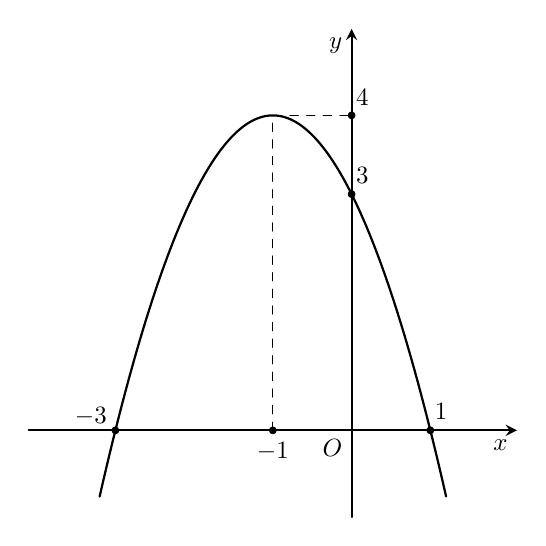
\begin{tikzpicture}[line join=round, line cap=round,>=stealth,thick]
					\tikzset{every node/.style={scale=0.9}}
					\draw[->] (-4.1,0)--(2.1,0) node[below left] {$x$};
					\draw[->] (0,-1.1)--(0,5.1) node[below left] {$y$};
					\draw (0,0) node [below left] {$O$};
					\draw[dashed,thin](-1,0)--(-1,4)--(0,4);
					\begin{scope}
						\clip (-4,-1) rectangle (2,5);
						\draw[samples=200,domain=-3.2:1.2,smooth,variable=\x] plot (\x,{-1*(\x)^2+-2*(\x)+3});
					\end{scope}
					\draw[fill=black] (1,0) circle (1pt) node[shift=(60:0.3)]{$1$};
					\draw[fill=black] (-3,0) circle (1pt)  node[shift= (150:0.4) ]{$-3$};
					\draw[fill=black] (-1,0) circle (1pt) node[shift=(-90:0.3)]{$-1$};
					\draw[fill=black] (0,4) circle (1pt)  node[shift= (60:0.3) ]{$4$};
					\draw[fill=black] (0,3) circle (1pt)  node[shift= (60:0.3) ]{$3$};
				\end{tikzpicture}
			\end{center}
		\end{itemize}
	}
\end{ex}

\begin{ex}[\textit{Trích đề thi HKI - Trường Chuyên Lê Hồng Phong năm học 2024 - 2025}]%[0D3H2-2]%[Dự án đề cương 2025]%[Đoàn Minh Tâm]
	Gọi $M$ và $m$ lần lượt là giá trị lớn nhất và giá trị nhỏ nhất của hàm số $y=-x^2+4 x+3$ trên đoạn $[0 ; 5]$. Khi đó $m+M$ bằng
	\loigiai{
		Ta có hàm số $ y=-x^2+4x+3 $ là hàm số bậc hai.\\
		Suy ra đồ thị hàm số là đường parabol có đỉnh là $ I(2;7)$.\\
		Do $ a=-1<0 $ nên bề lõm hướng xuống, ta có bảng biến thiên của hàm số trên $ [0;5] $ như sau
		\begin{center}
			
\begin{tikzpicture}[>=stealth]
				\tkzTabInit[nocadre=false,lgt=1,espcl=2,deltacl=0.5]{$x$/.7 ,$y$/2}
				{$0$ , $2$ , $5$}
				\tkzTabVar{-/$3$ , +/$7$ , -/$-2$}
			\end{tikzpicture}
		\end{center}
	Dựa vào bảng biến thiên ta có giá trị nhỏ nhất, giá trị lớn nhất của hàm số trên $ [0;5] $ lần lượt là $ -2 $ khi $ x=5 $ và là $ 7 $ khi $ x=2 $.\\
	Vậy $ M=7 $ và $ m=-2 $ nên $ M+m=7-2=5 $.
	}
\end{ex}

\begin{ex}[\textit{Trích đề thi HKI - Trường Phạm Quang Sáng - Năm học 2023-2024}]%[0D3H2-1]%[Dự án đề cương 2025]%[Đoàn Minh Tâm]
	Xác định giá trị $a$ và $b$ để đồ thị $(P)$ của hàm số $y=ax^2+bx+5$ có đỉnh $S(2;-3)$.
	\loigiai{Theo giả thiết, ta có
		\begin{eqnarray*}
			\heva{&S\in (P)\\&x_S=2}\Leftrightarrow \heva{&4a+2b+5=-3\\&-\dfrac{b}{2a}=2}\Leftrightarrow\heva{&4a+2b=-8 \\ &4a+b=0}\Leftrightarrow \heva{&a=2\\&b=-8.}
		\end{eqnarray*}
		Vậy $(P)\colon y=2x^2-8x+5$.}
\end{ex}

\begin{ex}%[0D3H2-1]%[Dự án đề cương 2025]%[Đoàn Minh Tâm]%[THPT Trần Quang Khải]
	Tìm công thức của hàm số bậc hai  có đồ thị như hình.
	\begin{center}
		\begin{tikzpicture}[>=stealth,line join=round,line cap=round,font=\footnotesize,scale=.8]
			\draw[->] (-2.5,0)--(4,0)node[below]{$x$};
			\draw[->] (0,-2.2)--(0,4.5)node[right]{$y$};
			\draw (0,0) node[below right] {$O$};
			\fill (-1,0)circle(0.03)node[above left]{$-1$}
			(3,0)circle(0.03)node[below]{$3$}
			(0,4)circle(0.03)node[left]{$4$}
			(1,0)circle(0.03)node[below]{$1$}
			(0,3)circle(0.03)node[left]{$3$};
			\draw[ domain=-1.5:3.5, samples=100] plot (\x,{-(\x)^2+2*\x+3});
			\draw[dashed] (1,0)|-(0,4);
		\end{tikzpicture}
	\end{center}


	\loigiai{
		Hàm số cần tìm có dạng $y=ax^2+bx+c$	 với $a<0$.\\
		Đồ thị hàm số đi qua $(-1;0)$, $(3;0)$, $(0;3)$ và $(1;4)$ nên
		$$\heva{&a-b+c=0\\&9a+3b+c=0\\&c=3\\&a+b+c=4}\Leftrightarrow \heva{&a=-1\\&b=2\\&c=3.}$$
		Vậy hàm số cần tìm là $y=-x^2+2x+3$.	}
\end{ex}

\begin{ex}[\textit{Trích đề thi HKI - Trường Phạm Văn Sáng - Năm học 2023-2024}]%[0D3H2-3]%[Dự án đề cương 2025]%[Đoàn Minh Tâm]
	Cho hàm số bậc hai $y=a x^2+b x+c$ $(a \neq 0)$ có đồ thị là parabol $(P)$. Biết rằng $(P)$ có đỉnh $I(1;3)$ và cắt trục tung tại điểm có tung độ là $ 4 $. Xác định $a$, $b$, $c$.
	\loigiai{
		Ta có $(P)$ cắt trục tung tại điểm có tung độ là 4 lên $c=4$. Khi đó, theo giả thiết
		\allowdisplaybreaks
		\begin{eqnarray*}
			\heva{
				&I \in (P) \\
				&x_I=-\dfrac{b}{2a}
			}
			\Leftrightarrow
			\heva{
				&a+b+4=3 \\
				&-\dfrac{b}{2a}=1
			} \Leftrightarrow
			\heva{&a+b=-1 \\
				&2a+b=0
			}
			\Leftrightarrow
			\heva{
				&a=1 \\ &b=-2.
			}
		\end{eqnarray*}
		Vậy $a=1$, $b=-2$ và $c=4$.
	}
\end{ex}

%D:\TeX\SP_TEX\SP344-Du_an_TEX-GK_10_11_dot_8\Sp đợt 8\data\10-TpHCM\0-TL-THPT-Phu-Nhuan-HCM-HKI-NH23-24.tex
\begin{ex}[\textit{Trích đề thi HKI - Trường Phú Nhuận - Năm học 2023-2024}]%[0D3V2-3]%[Dự án đề cương 2025]%[Đoàn Minh Tâm]
	Cho hàm số $f(x)=\heva{&2x-1&\text{khi}\ \ x<1\\&x^2-6x+6&\text{khi}\ \ x \geq 1.}$
	\begin{enumerate}
		\item Vẽ đồ thị hàm số $f(x)$.
		\item Tìm tất cả các giá trị của tham số $m$ sao cho phương trình $f(x)=m$ có $ 2 $ nghiệm phân biệt.
	\end{enumerate}
	\loigiai{
		\begin{enumerate}
			\item\immini{Vẽ đồ thị hàm số $f(x)$ như sau
			\begin{itemize}
				\item Với $ x<1 $, ta có $ f(x)=2x-1 $ là hàm số bậc nhất.\\
				Do đó, đồ thị của hàm số với $x \in (-\infty;1) $ là một đường thẳng
				Khi đó ta có bảng giá trị như sau
					\begin{center}
						\renewcommand\arraystretch{1.8} %độ rộng của hàng
						\begin{tabular}{c|c|c}
							$x$&$-1$&$0$\\
							\hline
							$f(x)$&$-3$&$-1$
						\end{tabular}
					\end{center}
				\item Với $ x\ge 1 $, ta có $ f(x)=x^2-6x+6 $ là hàm số bậc hai.\\
				Do đó, đồ thị của hàm số với $ x\in [1;+\infty) $ là đường parabol có đỉnh là $ I(3;-3) $.\\
				Bề lõm quay lên trên vì $a>0$, có trục đối xứng là $ x=3 $ và đi qua điểm $ A(1;1) $.
			\end{itemize}
			Khi đó, ta được hình vẽ bên.
			}{
			\begin{tikzpicture}[scale=.8, font=\footnotesize, line join=round, line cap=round,>=stealth]
				\def\a{1} \def\b{-6} \def\c{6} % Hệ số
				\def\xmin{-2.5} \def\xmax{6}
				\def\ymin{-4} \def\ymax{4}
				%	\draw[color=gray!50,dashed] (\xmin,\ymin) grid (\xmax,\ymax);
				\draw[->] (\xmin,0)--(\xmax,0) node [below]{$x$};
				\draw[->] (0,\ymin)--(0,\ymax) node [left]{$y$};
				\node at (0,0) [below left]{$O$};
				\node at (0,-2) [left]{$-2$};
				\draw[smooth,samples=300,domain=1:5.5] plot(\x,{\a*(\x)^2+\b*(\x)+\c});
				\draw[smooth,samples=300,domain=-1.6:1] plot(\x,{2*(\x)-1});
				\draw[dashed](1,0)node[below]{$1$}--(1,1)--(0,1)node[left]{$1$};
				\draw[dashed](3,0)node[above]{$3$}--(3,-3)--(0,-3)node[below left]{$-3$};
				\draw[dashed](-1,0)node[above]{$-1$}--(-1,-3)--(0,-3);
			\end{tikzpicture}		}
			\item Số nghiệm của phương trình $f(x)=m$ là số giao điểm của hai đồ thị $\heva{&y=f(x)\\&y=m}$ (vì $ d\colon y=m \parallel Ox $).\\
			Khi đó phương trình $f(x)=m$ có 2 nghiệm $\Leftrightarrow\hoac{&m=1 \\&m=-3.}$
		\end{enumerate}
	}
\end{ex}

\begin{ex}[\textit{Trích đề thi HKI - Trường Nguyễn Du - Năm học 2023-2024}]%[0D3H2-4]%[Dự án đề cương 2025]%[Đoàn Minh Tâm]
	Cho parabol $(P) \colon y=x^{2}-3 x+4$ và đường thẳng $d \colon y=x+4$. Gọi $A(m; n)$ là tọa độ giao điểm giữa $(P)$ và $d$. Tính giá trị $m^{2}-n$, cho biết điểm $A$ có hoành độ dương.
	\loigiai{
		Phương trình hoành độ giao điểm của parabol $(P)$ và đường thẳng $d$ là
		$$x^2-3x+4=x+4 \Leftrightarrow x^2-4x=0 	\Leftrightarrow \hoac{&x=0\\&x=4.}$$
		Vì $A$ có hoành độ dương nên tọa độ của điểm $A$ là $A(4;8)$.\\
		Vậy nên $m=4$, $n=8$ và do đó $m^2-n=16-8=8$.
	}
\end{ex}


\begin{ex}[\textit{Trích đề thi HKI - Trường Nguyễn Công Trứ - Năm học 2023-2024}]%[0D3H2-6]%[Dự án đề cương 2025]%[Đoàn Minh Tâm]
	Một nhóm học sinh thi xem ai phát cầu lông được xa hơn. Trong mặt phẳng toạ độ $Oxy$, chọn điểm có tọa độ $\left(0; y_0\right)$ làm điểm phát cầu thì phương trình quỹ đạo của quả cầu khi rời khỏi mặt vợt là $y=\dfrac{-g \cdot x^2}{2 \cdot v_0^2 \cdot \cos ^2 \alpha}+(\tan \alpha) \cdot x+y_0$. Trong đó $g=9{,}8\left(\mathrm{m} / \mathrm{s}^2\right)$ là gia tốc trọng trường; $\alpha$ là góc phát cầu (so với phương ngang của mặt đất); $v_0$ $(\mathrm{m} / \mathrm{s})$ là vận tốc ban đầu của quả cầu; $y_0$ (mét) là khoảng cách từ vị trí phát cầu đến mặt đất. Bạn Cường thực hiện lượt thi của mình với góc phát cầu bằng $45^{\circ}$, cầu rời mặt vợt ở độ cao $0{,}8$ $(\mathrm{m})$ và vận tốc ban đầu của cầu là $6$ $(\mathrm{m} / \mathrm{s})$ (bỏ qua sức cản của gió và xem quỹ đạo của cầu luôn nằm trong mặt phẳng thẳng đứng). Biết rằng thành tích tốt nhất của các bạn tham gia thi trước Cường là phát được một quả cầu rơi chạm đất ở vị trí cách nơi đứng phát quả cầu ấy một khoảng bằng $4{,}5$ $(\mathrm{m})$. Hỏi bạn Cường có vượt qua được thành tích đó hay không? Vì sao?
	\loigiai{
		Đặt $x$, $(x>0)$ là khoảng cách từ vị trí phát cầu đến điểm chạm đất. Khi cầu chạm đất, ta có phương trình
		$$y = 0\Leftrightarrow\frac{-9{,}8 \cdot x^2}{2 \cdot 6^2 \cdot \cos^2 45^{\circ}} + (\tan 45^{\circ}) \cdot x + 0{,}8 = 0$$
		Giải phương trình trên ta được $x \approx 4{,}35$ (m).\\
		Do đó bạn Cường không vượt qua được thành tích vì $4{,}35<4{,}5$.
	}
\end{ex}



\begin{ex}[\textit{Trích đề thi HKI - Trường Lê Trọng Tấn - Năm học 2023-2024}]%[0D3V2-6]%[Dự án đề cương 2025]%[Đoàn Minh Tâm]
	Chuyển động của một vật ném xiên nếu bỏ qua sức cản của không khí và gió thì độ cao $y$ (tính bằng mét) của vật so với điểm ném sẽ tuân theo phương trình  $y=\dfrac{-g}{2 v_0^2 \cos ^2 \alpha} x^2+x \tan \alpha$ trong đó $x$ là khoảng cách (tính bằng mét) vật bay được theo phương ngang tính từ điểm ném, vận tốc ban đầu $v_0$ của vật hợp với phương ngang một góc $\alpha$ và $g=9,8 \mathrm{~m} / \mathrm{s}^2$ là gia tốc trọng truờng.\\
	Một cầu thủ đá quả bóng lên từ mặt đất với vận tốc ban đầu $20$ m/s  và góc đá so với phương ngang là $45^{\circ}$ thẳng vào khung thành bị bỏ trống trước mặt cách $39 $ m. Hỏi cầu thủ đó có đưa bóng vào được khung thành không? Biết rằng mép dưới sà ngang của khung thành cao $2{,}44$ m so với mặt đất và bỏ qua sức cản của không khí và gió.
	\loigiai{
		Phương trình chuyển động của quả bóng là $$y=\dfrac{-9{,}8}{2\cdot 20^2 \cdot \cos ^2 45^\circ} x^2+x \tan 45^\circ =-\dfrac{49}{2000}x^2+x.$$
		Chiều cao của quả bóng cách vị trí quả bóng đá lên $39$ m là $y(39)=1{,}7355$ m.\\
		Vì chiều cao của quả bóng trước khung thành thấp hơn so với chiều cao của khung thành nên cầu thủ đưa bóng vào lưới.
	}
\end{ex}

\begin{ex}[\textit{Trích đề thi HK1 - Trường THTH Sài Gòn - Năm 2023-2024}]%[0D3V2-6]%[Dự án đề cương 2025]%[Đoàn Minh Tâm]%
	Nhân dịp Tết sắp đến, một cửa hàng bán đồ lưu niệm dự định thiết kế hàng loạt các sản phẩm bằng kính dày $5$ mm có khắc hình cành mai lên bề mặt như hình 1. Trước khi đi vào sản xuất, cửa hàng đã dự trù chi phí dựa trên việc tính toán diện tích một mặt $S$ của mỗi tấm kính theo công thức như hình 2. Biết rằng viền của tấm kính là một phần đồ thị của hàm số bậc hai như hình 3. Tính chi phí kính tối thiểu để làm một sản phẩm biết mỗi mét vuông kính dày $5$ mm có giá $220\,000$ đồng, bỏ qua sự hao hụt trong quá trình cắt kính (làm tròn kết quả đến hàng đơn vị).
	\begin{center}
		\begin{tabular}{c c c}
			\definecolor{green(pigment)}{rgb}{0.0, 0.65, 0.31}
			\definecolor{canaryyellow}{rgb}{1.0, 0.94, 0.0}
			\definecolor{gold}{rgb}{1.0, 0.84, 0.0}
			\definecolor{cadmiumred}{rgb}{0.89, 0.0, 0.13}
			\definecolor{brown(traditional)}{rgb}{0.59, 0.29, 0.0}
			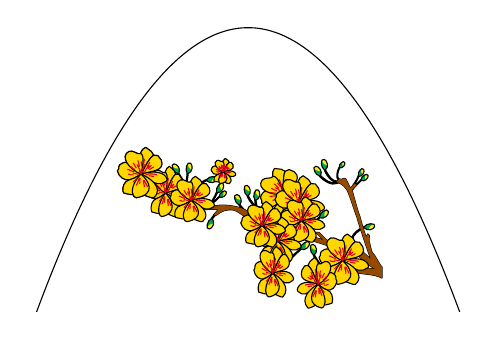
\begin{tikzpicture}[line join=round, line cap=round,scale=0.2,transform shape]
				\clip (-14,-6) rectangle (14,12);

				\tikzset{than/.pic={
						\def\Canh{
							(8.5,-3.2)
							..controls +(140:.2) and +(-40:.2) ..(7.9,-2.3)
							..controls +(150:.1) and +(-60:.1) ..(7.68,-1.58)
							..controls +(130:.1) and +(-80:.1) ..(7.7,-1.2)--(7.6,-1.1)--(7.5,-1.3)
							..controls +(130:.1) and +(-80:.1) ..(7.1,0)
							..controls +(130:.1) and +(-80:.1) ..(6.6,1.7)--(6.9,2)--(6.75,2.1)--(6.5,1.8)--(6.2,2.4)
							..controls +(140:.2) and +(-40:.2) ..(5.8,2.4)--(5.6,2.2)
							..controls +(-10:.2) and +(120:.2) ..(6.2,1.8)
							..controls +(-30:.2) and +(120:.2) ..(6.9,0)
							..controls +(-80:.2) and +(120:.2) ..(7.8,-2.7)
							..controls +(140:.2) and +(-50:.2) ..(6.6,-1.6)--(6.4,-1.6)--(6.6,-1.85)
							..controls +(160:.2) and +(-30:.2) ..(5,-1.5)--(4.5,-1)--(4.3,-1)--(4.8,-1.5)
							..controls +(160:.2) and +(-40:.5) ..(0,.3)
							..controls +(140:.6) and +(10:.5) ..(-2,.7)
							..controls +(-170:.6) and +(10:.5) ..(-4,.5)--(-4,.3)
							..controls +(10:.6) and +(160:.2) ..(-1.9,.45)--(-2.2,.1)--(-2,.1)
							..controls +(40:.6) and +(140:.6) ..(-.5,.2)
							..controls +(-40:1) and +(155:.8) ..(7,-2.5)
							..controls +(-40:.4) and +(155:.4) ..(8.2,-3.4)
							..controls +(150:.4) and +(-40:.2) ..(7,-3.2)--(6.8,-3.5)
							..controls +(-30:.4) and +(150:.6) ..(8.5,-3.9)--cycle

							;
						}
						\draw[black]\Canh;
						\fill[brown(traditional)] \Canh;
				}}

				\tikzset{bup1/.pic={
						\def\B1{
							(5.2,1.8)
							..controls +(-155:.1) and +(-50:.1) ..(4.6,2.6)
							..controls +(60:.3) and +(0:.2) ..(4.3,3.2)
							..controls +(-180:.3) and +(180:.2) ..(4.5,2.6)
							..controls +(-50:.5) and +(140:.1) ..(5,1.8)--cycle

							;
						}
						\fill[green(pigment)] \B1;

						\def\b1{
							(4.62,2.9)
							..controls +(65:.1) and +(0:.1) ..(4.3,3.2)
							..controls +(-180:.2) and +(180:.5) ..cycle
							;
						}
						\fill[canaryyellow] \b1;
						\draw[black]\B1;
				}}

				\tikzset{bup/.pic={
						\def\B{
							(5.6,2.2)
							..controls +(-155:.4) and +(-40:.4) ..(4.6,2.6)
							..controls +(60:.3) and +(0:.2) ..(4.3,3.2)
							..controls +(-180:.3) and +(180:.2) ..(4.5,2.6)
							..controls +(-50:.5) and +(-155:.3) ..(5.6,2.1)
							..controls +(25:.1) and +(-155:.1) ..(5.9,2.2)--cycle
							;
						}
						\fill[green(pigment)] \B;

						\def\b{
							(4.62,2.9)
							..controls +(65:.1) and +(0:.1) ..(4.3,3.2)
							..controls +(-180:.2) and +(180:.5) ..cycle
							;
						}
						\fill[canaryyellow] \b;
						\draw[black]\B;
				}}

				\tikzset{mai/.pic={
						\def\D{
							(-6.8,2.7)
							..controls +(80:.2) and +(-160:.7) ..(-6.5,4.4)
							..controls +(-30:.1) and +(150:.1) ..(-6.3,4.25)
							..controls +(0:.1) and +(120:.2) ..(-6,3.9)
							..controls +(-150:.4) and +(50:.2) ..cycle
							(-6.8,2.7)
							..controls +(20:.5) and +(120:.5) ..(-5.2,2.5)
							..controls +(-60:.3) and +(30:.3) ..(-5.5,2.1)
							..controls +(-150:.05) and +(30:.05) ..(-5.65,2.1)
							..controls +(-150:.05) and +(30:.05) ..(-5.8,2.1)
							..controls +(160:.8) and +(-35:.5) ..cycle
							(-6.8,2.7)
							..controls +(-150:.4) and +(10:.2) ..(-7.5,2.35)
							..controls +(-170:.4) and +(-75:.4) ..(-8.3,2.9)
							..controls +(40:.1) and +(-85:.1) ..(-8.2,3.2)
							..controls +(95:.1) and +(175:.1) ..(-7.8,3.45)
							..controls +(-5:.4) and +(145:.4) ..cycle
							;
						}
						\fill[gold] \D;
						\draw[black]\D;
						\def\C{

							(-6,3.9)
							..controls +(-150:.4) and +(50:.2) ..(-6.8,2.7)
							..controls +(20:.6) and +(-70:.8) ..(-5.52,3.6)
							..controls +(95:.05) and +(-30:.05) ..(-5.6,3.7)
							..controls +(95:.2) and +(0:.2) ..cycle

							(-6.8,2.7)
							..controls +(-20:.6) and +(40:.9) ..(-6,1.2)
							..controls +(-140:.1) and +(-10:.1) ..(-6.7,1.4)
							..controls +(170:.1) and +(-40:.1) ..cycle

							(-6.8,2.7)
							..controls +(-90:.6) and +(20:.6) ..(-7.3,1.4)
							..controls +(-160:.1) and +(-10:.1) ..(-7.9,1.5)
							..controls +(130:.1) and +(-80:.1) ..(-7.95,1.65)
							..controls +(100:.2) and +(-170:.4) ..(-7.5,2.35)
							..controls +(10:.2) and +(-150:.4) ..cycle

							(-6.8,2.7)
							..controls +(160:.8) and +(-155:.7) ..(-7.55,4.15)
							..controls +(-15:.3) and +(155:.7) ..(-7,4)
							..controls +(30:.1) and +(150:.1) ..(-6.8,4)
							..controls +(-30:.3) and +(80:.3) ..cycle
							;
						}

						\fill[gold] \C;
						\draw[black]\C;

						\def\T{
							(-6.8,2.7)
							..controls +(-40:.65) and +(10:1.3) ..(-7.1,1.2)
							..controls +(-170:.1) and +(-110:.05) ..(-7.3,1.4)
							..controls +(120:.4) and +(-140:.4) ..cycle
							;
						}
						\fill[gold] \T;
						\draw[black]\T;
						%============
						\def\V{
							(-6.8,2.7)
							..controls +(30:.1) and +(-130:.1) ..(-6.7,2.9)
							(-6.8,2.7)
							..controls +(30:.1) and +(-130:.1) ..(-6.8,3)
							(-6.8,2.7)
							..controls +(120:.1) and +(-30:.1) ..(-6.9,2.94)
							(-6.8,2.7)
							..controls +(150:.1) and +(-40:.1) ..(-6.9,2.85)
							;
						}
						\draw[cadmiumred]\V;
						%\fill[ecru!80] \V;
						%=================
						\def\N{
							(-7.3,3.4)
							..controls +(-40:.05) and +(140:.05) ..(-7.1,3.1)
							(-7.05,3.3)
							..controls +(-40:.05) and +(120:.05) ..(-6.9,3)
							(-7,3.55)
							..controls +(-40:.05) and +(120:.05) ..(-6.9,3.2)
							(-6.8,3.5)
							..controls +(-40:.05) and +(120:.05) ..(-6.75,3.2)
							(-6.6,3.3)
							..controls +(-40:.05) and +(100:.05) ..(-6.7,3)
							(-6.6,3.65)
							..controls +(-40:.05) and +(100:.05) ..(-6.65,3.3)
							(-6.3,3.25)
							..controls +(-40:.05) and +(100:.05) ..(-6.5,3)
							(-6.25,3.45)
							..controls +(-40:.05) and +(100:.05) ..(-6.4,3.2)
							(-6.35,3.05)
							..controls +(40:.05) and +(-150:.05) ..(-6.15,3.25)
							(-6.25,3)
							..controls +(40:.05) and +(-150:.05) ..(-6,3.15)
							(-6.3,2.6)
							..controls +(40:.05) and +(-150:.05) ..(-6,2.55)
							(-7.3,2.75)
							..controls +(40:.05) and +(-150:.05) ..(-7,2.7)
							(-7.6,2.7)
							..controls +(-40:.05) and +(-150:.05) ..(-7.3,2.65)
							(-7.65,3)
							..controls +(10:.05) and +(-150:.05) ..(-7.25,2.85)
							(-7.5,3.2)
							..controls +(10:.05) and +(-150:.05) ..(-7.2,3)
							(-7.3,2.2)
							..controls +(10:.05) and +(-150:.05) ..(-7.1,2.4)
							(-7.1,2)
							..controls +(10:.05) and +(-150:.05) ..(-6.9,2.45)
							(-6.9,2.1)
							..controls +(10:.05) and +(-150:.05) ..(-6.85,2.45)
							(-6.6,1.9)
							..controls +(10:.05) and +(-150:.05) ..(-6.65,2.3)
							(-6.4,1.9)
							..controls +(10:.05) and +(-150:.05) ..(-6.58,2.3)
							(-6.2,2.75)
							..controls +(-150:.05) and +(20:.05) ..(-6.5,2.65)
							(-6.2,2.7)
							..controls +(30:.05) and +(120:.05) ..(-5.8,2.65)
							(-6.65,2.8)
							..controls +(30:.05) and +(-100:.05) ..(-6.5,2.95)
							;
						}
						\draw[cadmiumred]\N;
				}}

				\path
				(0,0)pic[scale=1]{bup}
				(3.4,4.7)pic[scale=.8,rotate=-60]{bup1}
				(4.5,5.55)pic[scale=.8,rotate=-80]{bup1}
				(-.3,2.1)pic[scale=1,rotate=-20]{bup}
				(3,5.5)pic[scale=.7,rotate=-70]{bup}
				(-4.7,2)pic[scale=1,rotate=-40]{bup}
				(-5.5,-1)pic[scale=1,rotate=-10]{bup}
				(-5.2,.45)pic[scale=1,rotate=-20]{bup}
				(-7.25,1.62)pic[yscale=-1,scale=1,rotate=-10]{bup}
				(-6.5,4.2)pic[scale=1,rotate=-60]{bup1}
				(-9,3.7)pic[scale=1,rotate=-40]{bup1}
				(-9,.15)pic[scale=1]{bup1}
				(0,2)pic[scale=1,rotate=-80]{bup1}
				(1.2,4)pic[scale=1,rotate=-80]{bup1}
				(-1,-3.3)pic[scale=1,rotate=-20]{bup}
				(-3.5,7.5)pic[scale=1,rotate=-110]{bup}
				(6.5,4.5)pic[scale=1,rotate=-110]{bup}
				(-4.5,4.5)pic[scale=.8,rotate=-80]{bup1}
				;
				\path (0,0)pic[scale=1]{than}
				(0,0)pic[scale=1]{mai}
				(1.8,1.5)pic[scale=.5]{mai}
				(.2,-1.2)pic[xscale=.8]{mai}
				(0,0)pic[scale=1]{mai}
				(2.5,-1.4)pic[scale=.9]{mai}
				(9.5,2.5)pic[scale=1,rotate=30]{mai}
				(10,-1.8)pic[scale=1]{mai}
				(9.5,-2.7)pic[scale=.9]{mai}
				(8,-4)pic[scale=.9]{mai}
				(7,-3)pic[scale=.9]{mai}
				(7,-6.3)pic[xscale=.8]{mai}
				(12.8,-5.5)pic[scale=1]{mai}
				(-1,-7)pic[xscale=-.8,rotate=0]{mai}

				;
				\draw[smooth,samples=100,domain=-14:14] plot(\x,{-.1*(\x)^2+12});
				%\draw (12,8) node[above] {Hình 1};
			\end{tikzpicture}
			&
			\begin{tikzpicture}[scale=0.7, font=\footnotesize, line join=round, line cap=round, >=stealth]
				\def\xmin{-4}\def\xmax{4}\def\ymin{0}\def\ymax{6}
				\draw[<->] (2,0)--(2,4) node[midway, right] {\footnotesize $h$};
				\draw[<->] (0,0)--(4,0) node[midway, below] {\footnotesize $d$};
				\clip (-0.5,0) rectangle (4.2,6);
				\draw[smooth,samples=200,domain=\xmin:\xmax] plot (\x,{-1*((\x)^2)+4*(\x)});
				\draw (2,5.5) node[below] {$S=\dfrac{2}{3}hd$};
				%\draw (3,0.2) node[above] {Hình 2};
			\end{tikzpicture}
			&
			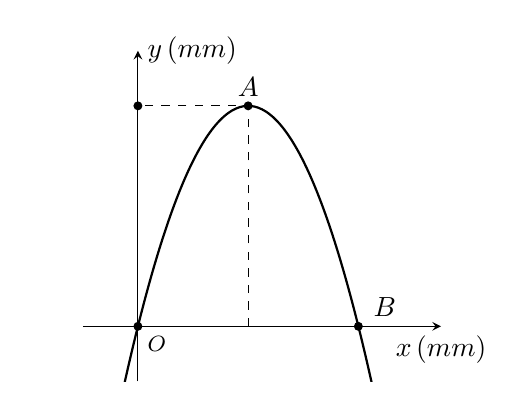
\begin{tikzpicture}[>=stealth,x=1cm,y=1cm,scale=0.7]
				\def\a{-1}
				\def\d{4}
				\def\b{-0.5}
				\def\c{1}
				\draw[->] (-1,0)--(5.5,0)node[below]{$x\left(\text{mm}\right)$};
				\draw[->] (0,-1)--(0,5)node[right]{$y\left(\text{mm}\right)$};
				\draw (0,0)node[below right]{\footnotesize $O$};
				\clip (-2,-1) rectangle(5.2,5);
				\draw[thick,samples=150,smooth,domain=-5:5] plot(\x,{\a*(\x)^2+\d*(\x)});
				\draw [dashed] (2,0)--(2,4)--(0,4);
				\draw (2,4) node[above]{$A$};
				\fill (4.1,0) node[above right]{$B$};
				\foreach \x/\y in {0/0,0/4,2/4,4/0}{\draw[fill=black] (\x,\y) circle (2pt);}
				%\fill (2,-1) node[below] {Hình 3};
			\end{tikzpicture}\\
			Hình 1 & Hình 2 & Hình 3
		\end{tabular}
	\end{center}
	\loigiai{
		Phương trình $-\dfrac{1}{25}x^2+4x=0\Leftrightarrow\hoac{&x=0\\&x=100}$ nên tọa độ điểm $B\left(100;0\right)$, tức $d=100$ mm.\\
		Tọa độ đỉnh của parabol là $A\left(50;100\right)$  nên $h=100$ mm.\\
		Vậy diện tích của mỗi tấm kính là $\dfrac{2}{3}\cdot100\cdot100 = \dfrac{20\,000}{3}$ mm$^2$  $= \dfrac{1}{150} $m$^2$.\\
		Chi phí sản xuất một tấm kính là $\dfrac{1}{150}\cdot220\,0000\approx1\,467$ đồng.
	}
\end{ex}


